% UGRC 2 report -- Aadi Srivastava (CS23B100), guide: KC Sivaramakrishnan.
% Build:  pdflatex main && bibtex main && pdflatex main && pdflatex main
%         (or: latexmk -pdf main.tex, or upload the report/ folder to Overleaf)
\documentclass[11pt,a4paper]{article}

\usepackage[T1]{fontenc}
\usepackage[utf8]{inputenc}
\usepackage{lmodern}
\usepackage[a4paper,margin=2.5cm,headheight=14pt]{geometry}
\usepackage{amsmath,amssymb}
\usepackage{graphicx}
\usepackage{booktabs}
\usepackage{tabularx}
\usepackage{multirow}
\usepackage{array}
\usepackage{longtable}
\usepackage[table]{xcolor}
\usepackage{enumitem}
\usepackage{caption}
\usepackage{subcaption}
\usepackage{float}
\usepackage{listings}
\usepackage{fancyhdr}
\usepackage{titlesec}
\usepackage{microtype}
\usepackage[hidelinks]{hyperref}
\usepackage{url}

\graphicspath{{figures/}}

% ---------------------------------------------------------------- colours
\definecolor{ugblue}{RGB}{31,63,127}
\definecolor{uggrey}{RGB}{128,128,128}
\definecolor{codebg}{RGB}{248,248,248}
\definecolor{codecomment}{RGB}{90,120,90}
\definecolor{codekw}{RGB}{31,63,127}
\definecolor{rowhi}{RGB}{232,239,250}
\hypersetup{colorlinks=true,linkcolor=ugblue,citecolor=ugblue,urlcolor=ugblue}

% ---------------------------------------------------------------- headings
\titleformat{\section}{\normalfont\Large\bfseries\color{ugblue}}{\thesection}{1em}{}
\titleformat{\subsection}{\normalfont\large\bfseries\color{ugblue}}{\thesubsection}{1em}{}
\titleformat{\subsubsection}{\normalfont\normalsize\bfseries\color{ugblue}}{\thesubsubsection}{1em}{}

% ---------------------------------------------------------------- running header
\pagestyle{fancy}
\fancyhf{}
\renewcommand{\sectionmark}[1]{\markboth{\thesection\quad #1}{}}
\fancyhead[L]{\small\MakeUppercase{\leftmark}}
\fancyhead[R]{\small UGRC 2 Report}
\fancyfoot[C]{\thepage}
\renewcommand{\headrulewidth}{0.4pt}

% ---------------------------------------------------------------- listings
\lstdefinelanguage{OCamlX}{
  morekeywords={let,in,for,to,downto,do,done,if,then,else,match,with,fun,
    function,mutable,type,module,open,external,rec,and,begin,end,while,of},
  sensitive=true,
  morecomment=[n]{(*}{*)},
  morestring=[b]"
}
\lstdefinelanguage{CmmX}{
  morekeywords={let,letmut,catch,exit,with,if,load,store,alloc,poll,assign},
  sensitive=true,
  morecomment=[l]{;}
}
\lstdefinelanguage{asmX}{
  morekeywords={mov,movsd,vmovsd,vmulsd,vaddsd,vfmadd231sd,vfmadd231pd,
    vmovupd,addsd,mulsd,add,sub,cmp,jl,jle,jg,jge,jne,je,jmp,lea,sar,shl,inc,
    dec,test,call,ret,cmpq,addq,movq,leaq,subq,sarq,jb,jae,ja,jbe,nop,
    vxorpd,vaddpd,vmulpd,vfmadd213sd,imul},
  sensitive=false,
  morecomment=[l]{\#}
}
\lstdefinelanguage{plaintext}{}
\lstset{
  basicstyle=\ttfamily\footnotesize,
  keywordstyle=\color{codekw}\bfseries,
  commentstyle=\color{codecomment}\itshape,
  stringstyle=\color{teal},
  numbers=left,
  numberstyle=\tiny\color{uggrey},
  numbersep=6pt,
  backgroundcolor=\color{codebg},
  frame=single,
  rulecolor=\color{black!15},
  breaklines=true,
  columns=fullflexible,
  keepspaces=true,
  showstringspaces=false,
  tabsize=2,
  captionpos=b,
  xleftmargin=1.5em,
  framexleftmargin=1.5em,
  aboveskip=0.8em,
  belowskip=0.6em
}
\renewcommand{\lstlistingname}{Listing}

% ---------------------------------------------------------------- misc
\setlist{itemsep=2pt,topsep=4pt}
\captionsetup{font=small,labelfont=bf}
% \code{...} prints its argument verbatim in typewriter (underscores allowed).
% Do not use it in captions or section titles; write \texttt{a\_b} there.
\newcommand{\code}[1]{\texttt{\detokenize{#1}}}
% \ainl|...| prints inline assembly verbatim, including % and $ characters.
\newcommand*{\ainl}{\lstinline[basicstyle=\ttfamily\small,language=plaintext]}
% \reg{r11} prints the register name %r11.
\newcommand{\reg}[1]{\texttt{\%#1}}
\newcommand{\x}{\ensuremath{\times}}
\setlength{\parskip}{0.35em}
\renewcommand{\arraystretch}{1.12}

\begin{document}

% ================================================================ title page
\begin{titlepage}
  \centering
  \vspace*{4cm}
  {\color{ugblue}\Huge\bfseries Mind the Gap:\\[0.3em]
   Porting a Transformer Across Languages\\[0.3em]
   and Teaching OxCaml to Catch Up with C++\par}
  \vspace{1.6cm}
  {\large UGRC 2 : Aadi Srivastava CS23B100\par}
  \vspace{0.4cm}
  {\large Guide: KC Sivaramakrishnan\par}
  \vspace{0.6cm}
  {\color{uggrey}\small Performance Engineering $\cdot$ Optimising Compilers $\cdot$
    Garbage-Collected Runtimes $\cdot$ OCaml / OxCaml\par}
  \vspace{2.5cm}
  \rule{0.45\textwidth}{0.4pt}
  \vfill
\end{titlepage}

\tableofcontents
\clearpage

\section{Introduction and Project Motivation}
\label{sec:intro}

Machine learning is written in Python and made fast in C++. OxCaml~\cite{oxcaml},
Jane Street's performance-oriented branch of OCaml, is built to test whether a
high-level, garbage-collected, type-safe language can run close to C++ when the
programmer can \emph{opt in} to performance. This project asks a narrow,
measurable version of that question: running one small language model's
inference on a single CPU core in five languages that compute the same thing
under one numerical contract, \emph{where does OCaml lose time to C++, and how much can be won
back in the source, the runtime and the compiler?}

The workload is Andrej Karpathy's \code{microgpt.py}~\cite{karpathy_microgpt},
a dependency-free GPT trained on 32,032 first names~\cite{karpathy_makemore}.
I ported its inference to C++, Rust, OCaml and OxCaml, built a benchmark that
checks the ports agree in every printed digit, and then closed the gap between
OxCaml and C++, each step chosen by what the previous one measured.

\subsection{Initial Approach: Novel CPU Inference in llama.cpp}
\label{sec:intro-llamacpp}

The first three weeks of August went into looking for a novel change to CPU
inference in \code{llama.cpp}~\cite{llamacpp}, the standard C/C++ engine for
running language models on CPUs.

\paragraph{KV-cache compression.} The first proposal was to compress cold
key--value cache entries on idle cores during decoding. Following my guide's
suggestion, I first implemented existing schemes: StreamingLLM-style
eviction~\cite{xiao2024streamingllm} and a reformulation of KIVI's per-channel
key quantisation~\cite{liu2024kivi}. Evicting one token per step made decoding
42\% \emph{slower}, and batched eviction was still 11\% slower despite 69\%
fewer resident tokens, because attention scans the cache's \emph{physical} span
and \code{llama.cpp} never compacts the holes that eviction leaves.

\paragraph{Algorithmic ideas.} Eight further ideas (activation sparsity,
speculative decoding, Barnes--Hut style summaries of KV pages, prefetching, and
others) were each ruled out by a cheap measurement of their assumption: for
example, only 0.7\% of feed-forward neurons can be skipped in blocks of 64,
although 32\% are individually inactive.

\paragraph{A focused workload.} In a heavily optimised engine a new idea is
either prior art or quickly settled by measurement. The project therefore
moved to a workload small enough to understand instruction by instruction,
where the variable is the \emph{language and its compiler}, measured with a
paired, pinned, interleaved protocol (Section~\ref{sec:method}).

\subsection{Core Goals}
\begin{itemize}
  \item Port microgpt inference to four languages with \emph{bit-identical}
        output, verified by a hash.
  \item Measure throughput fairly, each optimisation a separate build variant.
  \item Find at the instruction level why OCaml is slower than C++, and close
        the gap in the source, the runtime and the OxCaml compiler.
  \item Check that the compiler changes generalise, on a numerical library
        (nx-oxcaml) and a cryptography code base (oxcaml-crypto-study).
\end{itemize}

\subsection{Summary of Outcomes}
All gaps are throughput of non-vectorised C++ divided by throughput of the
OCaml build, from one benchmark run (Section~\ref{sec:runu}) on the OxCaml
5.4.0-ox7 release. The first OxCaml port was $4.19\times$ slower
than C++; removing bounds checks and unrolling brought it to
$1.65\times$. Most of the remaining gap was integer address
arithmetic in one loop: OCaml cannot form pointers into the middle of an
array, and the OxCaml optimiser has no loop optimisations.

I added four passes over OxCaml's Cmm intermediate language --- strength
reduction, interior pointers, invariant-stride induction variables and
loop-invariant code motion (LICM) --- and \emph{counted loops}, which poll
once on exit instead of on every back edge when termination is proved, so the
pointer passes can act with polls on. On the pull-request
compiler~\cite{oxcaml_pr}, rebased onto OxCaml's main branch, they speed up
the unchanged source by \textbf{$+30.2\%$ (21/21)} over the same
compiler with the passes off, and by $+29.2\%$ (21/21) over
the release. With bounds checks
off, a hand-unrolled kernel and \code{-cmm-counted-loops}, OxCaml runs at
$1.29\times$ scalar C++ ($1.40\times$ vectorised C++); bounds-checked
Rust is at $1.02\times$. With bounds checks kept, the pull request is
\emph{slower} than the release, $-14.9\%$ (1/21). The collector never sees a derived pointer and
every proved loop reaches its exit poll, but how long another domain waits for
that poll is not bounded; that latency is the cost.

Strength reduction and LICM are textbook, with OCaml-specific cost rules;
counted loops adapt HotSpot C2's safepoint elision to an ahead-of-time
compiler; the OCaml-specific part is confining derived pointers to loop
regions in which no object can move (Section~\ref{sec:related}). With default
flags the test suite gives the same result as an unpatched build. Over passes
off, counted loops speed up nx-oxcaml's element-wise kernels by
$1.4$--$2.4\times$, and PolyBench kernels by $19.7\%$ with compile-time sizes
and $7.5\%$ with sizes known only at run time; ported to stock OCaml 5.3.0,
the passes gain $+17.6\%$ (21/21). They do nothing
for ChaCha20 (Section~\ref{sec:generality}). Figure~\ref{fig:timeline} shows
the journey.

\begin{figure}[t]
  \centering
  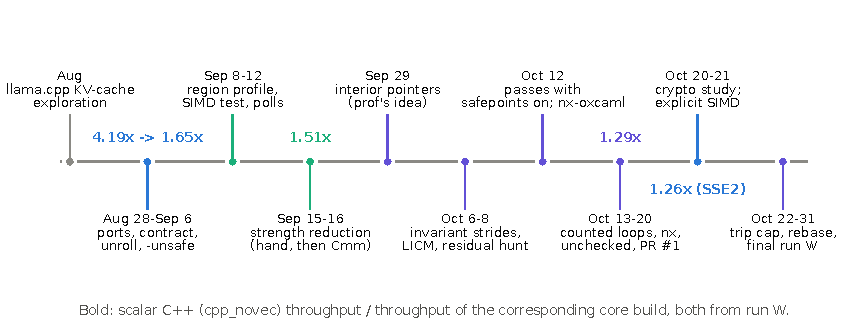
\includegraphics[width=\textwidth]{diag_timeline}
  \caption{Project timeline. Milestones show what was tried and, where a core
  build of run W corresponds, its gap to scalar C++.}
  \label{fig:timeline}
\end{figure}

\section{Background}
\label{sec:background}

\subsection{The microgpt Model}
\label{sec:model}

microgpt is a one-layer decoder-only transformer~\cite{vaswani2017attention}
in the GPT-2 style~\cite{radford2019gpt2}, simplified in three ways: RMSNorm
without a learned gain instead of LayerNorm~\cite{zhang2019rmsnorm}, no biases,
and ReLU instead of GeLU. Table~\ref{tab:model} lists its shape. I trained it
once (1,000 Adam steps, loss $3.37 \to 2.32$) and exported the weights to a
binary file that every port reads.

\begin{table}[h]
  \centering
  \small
  \begin{tabular}{@{}ll@{\hspace{2.2em}}ll@{}}
    \toprule
    layers & 1 & vocabulary & 27 (26 letters + BOS) \\
    embedding width & 16 & context length & 16 tokens \\
    heads $\times$ head width & $4 \times 4$ & MLP hidden width & 64 \\
    normalisation & RMSNorm, $(\overline{x^2} + 10^{-5})^{-1/2}$ & parameters & 4,192 (f64) \\
    \bottomrule
  \end{tabular}
  \caption{microgpt hyperparameters.}
  \label{tab:model}
\end{table}

One function, \code{linear}, applies all weight matrices
(Figure~\ref{fig:forward}): a matrix--vector product whose outputs are dot
products of a weight row with the input. Its 3,504 multiply--accumulates (MACs)
per token are over 90\% of the model's arithmetic, so it is the hot loop.

\begin{figure}[h]
  \centering
  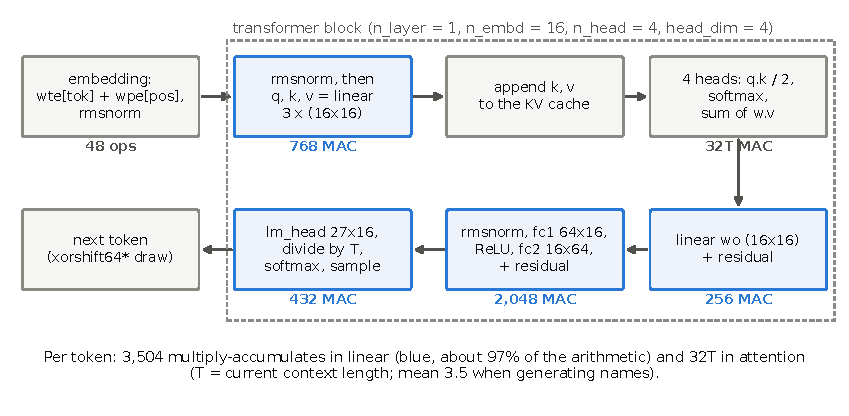
\includegraphics[width=\textwidth]{diag_forward}
  \caption{One microgpt forward pass. Blue boxes call \texttt{linear}, with
  their multiply--accumulate counts.}
  \label{fig:forward}
\end{figure}

The model's 33.5 KB of weights fit in the 48 KB L1 data cache, so the
benchmark measures per-operation overhead, not memory bandwidth.

\subsection{OCaml Values, Arrays and Bounds Checks}
\label{sec:ocaml-values}

OCaml uses a uniform value representation~\cite{minsky2022rwo}: a value is one
machine word, either an integer tagged in its least significant bit ($n$ is
stored as $2n+1$) or a pointer to just after a heap block's header word. A
\code{float array} stores unboxed 8-byte doubles, so a row-major weight matrix
has the layout of a C \code{double[]}.

Indexing \code{a.(i)} is bounds-checked unless compiled with \code{-unsafe}.
Tagged indices are free: for index $2i+1$, the byte offset $8i = 4(2i+1) - 4$ is
computed by the x86 addressing mode \code{-4(base,index,4)}.

\subsection{Garbage Collection and Safepoint Polls}
\label{sec:gc-polls}

OCaml's garbage collector is precise and moving: a minor collection copies live
objects and updates every pointer to them. With
\emph{domains}~\cite{sivaramakrishnan2020retrofitting}, minor collections are
stop-the-world: a domain needing one waits until every other domain reaches a
\emph{safepoint}. Allocations and calls are safepoints; a loop with neither
could run for ever, so the compiler puts a \emph{poll} on the back edge of any
loop it cannot prove safe:

\begin{lstlisting}[language=asmX,caption={A GC safepoint poll on x86-64: compare the young-heap pointer (\%r15) with the limit stored in the domain state (\%r14). The runtime raises the limit above any heap address to request a safepoint, so the next comparison takes the branch.},label=lst:poll,numbers=none]
cmpq   (%r14), %r15        # young_ptr vs young_limit
jbe    .Lcall_gc           # limit raised -> enter the runtime
\end{lstlisting}

Polls let signals be handled and other domains' collections make progress.
Single-domain programs such as microgpt do not need them, and OxCaml offers
\code{-disable-poll-insertion}, but removing polls from a multi-domain program
can deadlock it. This tension drives the second half of the project.

\subsection{Interior Pointers}
\label{sec:bg-interior}

A C++ kernel walks a pointer to each row. OCaml cannot: a pointer into the
middle of an array has no header, so the GC could neither tell which block it
belongs to nor update it when the block moves (Figure~\ref{fig:layout}), and
every access \code{d.(b1 + i)} recomputes \code{b1 + i}. The compiler's
\emph{derived} pointers (Cmm type \code{Addr}) may never be live where a
collection can happen, or the compiler stops with \code{bad GC root}.

\begin{figure}[h]
  \centering
  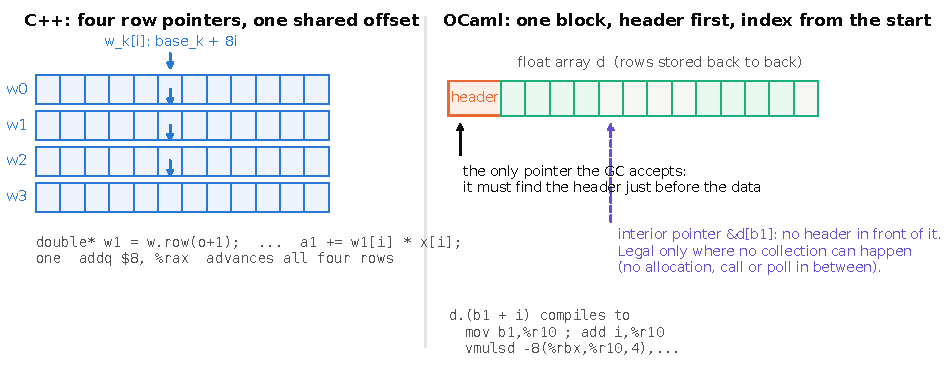
\includegraphics[width=\textwidth]{diag_layout}
  \caption{Left: C++ walks four row pointers with one shared offset. Right: an
  OCaml \texttt{float array} keeps its header in front of the data; a pointer
  into a row is legal only where no collection can happen.}
  \label{fig:layout}
\end{figure}

Other collected systems record at every safepoint how to recompute derived
pointers from their base~\cite{diwan1992compiler, llvm_statepoints}; OCaml's
frame tables have no such entries.

\subsection{OxCaml and the flambda2 Pipeline}
\label{sec:bg-pipeline}

OxCaml~\cite{oxcaml} extends OCaml with unboxed types, stack allocation, modes
and SIMD intrinsics, and replaces the classic optimiser with \emph{flambda2}.
After flambda2 the pipeline translates to \emph{Cmm} (a first-order language
in which a loop is a recursive \code{catch} whose parameters are the
loop-carried values), builds a control-flow graph, inserts safepoint polls,
allocates registers and emits assembly. Stock OCaml uses the older
\emph{closure} middle end. Section~\ref{sec:method} lists the compilers used.

\subsection{Instruction-Level Parallelism}
\label{sec:bg-ilp}

A dot product \code{acc += w[i] * x[i]} is a chain of dependent floating-point
additions, each waiting several cycles for the previous
one~\cite{fog_tables}. Computing four output rows at once gives the core four
independent chains to overlap (Figure~\ref{fig:ilp}); each row still adds its
terms left to right, so the result is bit-identical. An out-of-order core can
already overlap consecutive rows' chains, so the gain depends on how much
overlap the original loop allowed.

\begin{figure}[h]
  \centering
  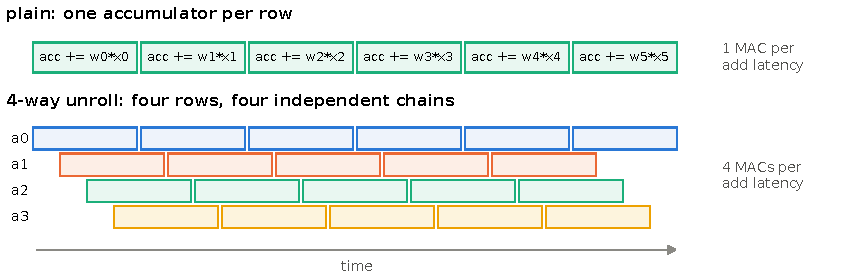
\includegraphics[width=0.92\textwidth]{diag_ilp}
  \caption{One chain of dependent additions versus four, one per output row;
  each row's summation order is unchanged.}
  \label{fig:ilp}
\end{figure}

\subsection{Related Work}
\label{sec:related}
Strength reduction of induction variables is
classical~\cite{cocke1977strength,allen1981strength}, and LLVM implements it in
\code{loop-reduce} and
\code{indvars}~\cite{llvm_passes}; LICM is textbook~\cite{aho2006dragon}. What
is specific here are the cost decisions for OCaml's tagged integers and
x86 addressing (Section~\ref{sec:sr-pass}).

Collected languages bound the time to a safepoint in several ways. OCaml
inserts polls since its safepoints work~\cite{ocaml_safepoints}; GHC omits
yield points in non-allocating loops unless \code{-fno-omit-yields} is
given~\cite{ghc_yields}. HotSpot's C2 compiler omits the back-edge safepoint of
\code{int} counted loops (\code{UseCountedLoopSafepoints}) and bounds the
resulting latency by \emph{strip mining}: an outer polled loop around counted
strips of \code{LoopStripMiningIter} iterations~\cite{jdk_stripmining}.
Graal's \code{LoopSafepointEliminationPhase} removes back-edge safepoints from
short counted loops~\cite{graal_safepoints}.

My counted loops follow C2's design, adapted to an ahead-of-time compiler: a
polled fallback copy, chosen by one check on entry, replaces deoptimisation,
and the termination proof is exact in wrapping arithmetic. The OCaml-specific
part is confining derived pointers to loop regions the collector cannot
enter, since OCaml's frame tables cannot describe them
(Section~\ref{sec:bg-interior}).

\section{Porting microgpt to Five Languages}
\label{sec:porting}

\subsection{The Ports}
A plain-float Python reference (\code{impl/python/infer.py}) matches the
original's autograd forward pass to a largest relative difference of
$1.26\times10^{-13}$ over 9,585 logits, and specifies the other four ports
(Table~\ref{tab:ports}). Every port is dependency-free, so the benchmark
compares languages, not libraries.

\begin{table}[h]
  \centering
  \small
  \begin{tabularx}{\textwidth}{@{}lXrl@{}}
    \toprule
    port & compiler and flags (benchmark) & lines & notes \\
    \midrule
    Python & CPython 3.13.5 & 480 & reference; explicit loops, no NumPy \\
    C++ & g++ 14.2, \code{-O3 -fno-fast-math} \code{-ffp-contract=off} & 845 & raw row pointers \\
    Rust & rustc 1.98.1, \code{--release} & 1,095 & safe Rust, iterator kernels \\
    OCaml & stock ocamlopt 5.3.0 (closure), \code{-unsafe} & 791 & same program as OxCaml$^\dagger$ \\
    OxCaml & OxCaml ocamlopt 5.4.0-ox7 (flambda2), \code{-O3 -unsafe} & 782 & same program as OCaml$^\dagger$ \\
    \bottomrule
  \end{tabularx}
  \caption{The five ports. Line counts include weight loading, harness and
  JSON reporting (the model is about 115 lines). $^\dagger$One program in
  standard OCaml; the two files differ only in comments and port-name strings,
  and the build refuses to proceed if they drift apart.}
  \label{tab:ports}
\end{table}

That program uses no OxCaml language extensions, so any difference between
the two rows is a difference between compilers; the only OxCaml-specific code
is the optional SSE2 kernel of Section~\ref{sec:simd}. Weights live in one
flat \code{float array} per matrix and accumulators are \code{float ref}s,
which both compilers keep unboxed. Allocation is 12.9 words per forward pass,
so the 256k-word minor heap fills only about once every 20,000 forward passes.

\subsection{A Bit-Exact Numerical Contract}
\label{sec:contract}

Agreement ``within a tolerance'' is too weak to catch porting bugs, so a
contract (\code{BENCHMARK.md}) pins every operation whose result could differ:

\begin{itemize}
  \item all arithmetic in \code{f64}; sums accumulated left to right in a plain
        loop, never compensated or pairwise; no fused multiply--add and no
        fast-math (\code{-ffp-contract=off}, no \code{mul_add});
  \item RMSNorm scale as \code{pow(ms + 1e-5, -0.5)} and attention scale as
        \code{pow(head_dim, 0.5)}, never \code{1/sqrt};
  \item ReLU written \code{x > 0 ? x : 0} (which maps NaN to 0), and logits
        divided by the temperature rather than multiplied by its reciprocal;
  \item sampling with a portable xorshift64*
        generator~\cite{marsaglia2003xorshift,vigna2016xorshift} and an ascending
        cumulative-sum scan with a strict \code{<} comparison.
\end{itemize}

Each run reports a perplexity over 2,000 held-out names (14,307 tokens), an
FNV-1a 64-bit hash~\cite{fnv} of all generated text, weight checksums and the
first four random numbers. The harness refuses to rank any port whose
checksums, draws or hash differ, or whose perplexity differs by more than
$10^{-9}$ relative. All five ports give the same perplexity in all 17
printed digits, $10.789614873329409$ (better than a bigram model's 12.33, a unigram model's
17.00 and the uniform 27.00) and the same hash, \code{0xae6c6ffbd8f5b02c}, for 200
samples. The logits themselves are not compared bit by bit, so these checks
make a difference in their last bits very unlikely but do not exclude it.

\subsection{Pitfalls the Contract Rules Out}
\label{sec:traps}

Several ordinary idioms change the last bit of the result, or the order of
side effects, in one language but not another (Table~\ref{tab:bugs}).

\begin{table}[h]
  \centering
  \small
  \begin{tabularx}{\textwidth}{@{}lXX@{}}
    \toprule
    language & pitfall & rule \\
    \midrule
    Python & \code{sum()} in CPython $\geq$ 3.12 uses Neumaier compensated summation~\cite{neumaier1974,python312sum}, more accurate than the other ports (Section~\ref{sec:challenges}) & explicit left-to-right loops \\
    Rust, C++ & \code{if x <= 0 {x = 0}} keeps NaN, because \code{NaN <= 0} is false & ReLU written \code{x > 0 ? x : 0} \\
    all & summing the loss per token or per document differs ($10^{-16}$) & accumulate per document, then add \\
    OCaml & \code{Array.init} leaves its call order unspecified, which matters when reading the weight file or drawing random numbers & explicit loops wherever order matters \\
    \bottomrule
  \end{tabularx}
  \caption{Idioms that make ports diverge silently; none changes the generated
  text.}
  \label{tab:bugs}
\end{table}

\section{Benchmark Methodology}
\label{sec:method}

\subsection{Machine}
All experiments ran on a laptop with an Intel Core Ultra 7 155H (6 performance,
8 efficiency and 2 low-power cores; AVX2), running a Debian environment under
WSL2 on Windows~11. Performance is attributed with \code{rdtsc} region
timers, instruction counts, disassembly and controlled experiments.

\subsection{Getting Numbers One Can Trust}
A hybrid CPU can move a long single-threaded job between core types and clock
levels, so every measurement follows one protocol, after~\cite{georges2007rigorous,mytkowicz2009wrong}:

\begin{enumerate}
  \item \textbf{Equal time, not equal work.} A measurement runs the forward
        pass repeatedly for 0.3\,s, three times in a fresh process, and keeps
        the fastest.
  \item \textbf{Pinning.} Every binary is pinned to one logical CPU
        (\code{taskset -c 0}).
  \item \textbf{Interleaved rounds.} Each of 21 rounds measures every variant
        once, so slow drift affects all variants equally. Tables report the
        median over rounds.
  \item \textbf{Paired deltas.} An optimisation's effect is the median of its
        per-round percentage change against the build it modifies, with the
        rounds it won (``+12.2\%, 21/21'') and, where the effect is small, the
        interquartile range.
  \item \textbf{Correctness first.} Every variant passes the output gate of
        Section~\ref{sec:contract} before any timing is accepted.
\end{enumerate}

Throughput is in tokens per second. \emph{Generation} mode, the default, times
the forward passes that sample 200 names from a fixed seed; \emph{scoring}
mode times those that compute the perplexity over the 14,307 held-out tokens.

\subsection{One Run for Every microgpt Number}
\label{sec:runu}
Absolute throughput drifts by 10--20\% between days, so every microgpt
throughput number in Sections~\ref{sec:stage1} to~\ref{sec:results} comes
from \textbf{one run}, called run~W: 62 builds measured on 31 October 2026 on
the same laptop, idle, after a five-minute settle, in 21 interleaved rounds in
both modes, all with identical output.

A typical variant's throughput varies by about 8\% between rounds
(interquartile range), which is why every comparison is paired within rounds.
As a built-in control, two byte-identical copies of one binary were measured
as different variants. They differed by $+0.6\%$
(median of the per-round differences, interquartile range
$[-0.2, +2.9]\%$, 15/21 rounds), so
differences between builds of less than about 3\% are treated as
indistinguishable.

\paragraph{Compilers.} The OxCaml release is 5.4.0-ox7 (opam
\code{oxcaml-compiler.5.4.0-ox7}), configured as its opam recipe does
(flambda2, poll insertion; Listing~\ref{lst:config}). The pull-request
compiler is commit \code{91acf6b} of branch
\code{ugrc2-rebased}~\cite{oxcaml_pr}: OxCaml main commit \code{327965f0e}
(30 October 2026) plus the pull request's 24 patches, configured the same
way. The series is also in the report's \code{data/pr-patches} directory; the
pull request's page shows an earlier revision of it. Stock
OCaml is 5.3.0 (commit \code{1ccb919}); \code{ocaml_pr_*} builds use it with
the same passes ported (five commits, a separate series that is not part of
the OxCaml pull request). Side results come from the previous release
5.2.0+ox (\code{oxcaml52_*}) and from the one-compiler-per-pass ladder of
Sections~\ref{sec:sr}--\ref{sec:stage6} (\code{ox54_*}), built on the
September 2026 main branch without poll insertion.

Table~\ref{tab:runs} lists the other experiments; each was made on the
compiler of its time and predates the final rebase.

\begin{table}[h]
  \centering
  \small
  \begin{tabularx}{\textwidth}{@{}lXl@{}}
    \toprule
    run & what it measures & rounds \\
    \midrule
    W & every microgpt build (62 variants), both modes; Sections~\ref{sec:stage1}--\ref{sec:results} & 21 \\
    regions & instrumented region profiles (Figure~\ref{fig:regions}) & 7 \\
    width & microgpt widths 32--256; \code{linear} in and out of cache (Section~\ref{sec:width}) & 21 \\
    nx & nx-oxcaml benchmarks (Sections~\ref{sec:nx-first} and~\ref{sec:counted}) & 13--21 \\
    PolyBench & 17 PolyBench kernels in OCaml and C (Section~\ref{sec:polybench}) & 21 \\
    crypto & ChaCha20 in oxcaml-crypto-study (Section~\ref{sec:crypto}) & 15 \\
    kernels & eight-row and index-form kernels (Sections~\ref{sec:sr} and~\ref{sec:simd-why}) & 21 \\
    layout & three builds at four code addresses (Section~\ref{sec:last2}) & 21 \\
    latency & two-domain safepoint-latency tests, without and with a trip cap (Section~\ref{sec:counted}) & 3 \\
    loops & inner loops timed alone, \code{llvm-mca} model (Section~\ref{sec:residual}) & 21 \\
    micro & one-off single-loop experiments (\reg{r11} patch, unconditional LICM, isolated shapes, hand-written loops, attention) & varies \\
    PR checks & final pull-request compiler: nx default flags, carried-value cap, trip-cap cost (Sections~\ref{sec:sr-pass} and~\ref{sec:counted}) & 15 \\
    tests & upstream test suites in three modes, adversarial programs, OCaml 5.3.0 port (Sections~\ref{sec:counted} and~\ref{sec:stock}) & --- \\
    \bottomrule
  \end{tabularx}
  \caption{Measurements behind the report, each with its own protocol. All
  except run W and the last two rows predate the final rebase.}
  \label{tab:runs}
\end{table}

\subsection{Variants and the Fair Baseline}
Every optimisation is a build switch, not a source edit. Variant names give
the language, safety (\code{safe} keeps bounds checks, \code{unsafe} uses
\code{-unsafe}), kernel (\code{plain} or four-row \code{unroll}) and
modifiers: \code{_sr} carries row indices by hand (Section~\ref{sec:sr});
\code{_pollfree} uses \code{-disable-poll-insertion} and \code{_pollnop}
overwrites the polls in the binary (Section~\ref{sec:polls}). \code{pr_*}
builds use the pull-request compiler: \code{pr_off} has the passes off,
\code{pr_all} the default flags (passes on, polls on every back edge), and
\code{pr_counted} adds \code{-cmm-counted-loops}; the ladder
\code{pr_c_off}, \code{pr_c_sr}, \code{pr_c_ip}, \code{pr_c_ivs} turns
counted loops on first and then adds one pass at a time
(Table~\ref{tab:passes}).

Main tables and figures show a core set: the C++, Rust and Python ports,
three stock OCaml builds, the source-level OxCaml stages on the release, the
pull-request ladder and \code{pr_simd_counted}. Builds that give up liveness
are shown apart (Table~\ref{tab:liveness}); others appear in the text.

The shipped C++ build is auto-vectorised by GCC (two rows per SSE2 register,
preserving each row's summation order); no OCaml variant vectorises until
Section~\ref{sec:simd}. C++ compiled with \code{-fno-tree-vectorize}
(\code{cpp_novec}) executes the same four scalar chains as the OCaml kernel:
it is the \emph{fair baseline}. Gaps quoted as ``$n\times$'' are
$\text{throughput}(\texttt{cpp\_novec}) / \text{throughput}(\text{OCaml variant})$
unless stated otherwise.

All code, build scripts and benchmark tools are in the project
repository~\cite{llamaport_repo} at tag \code{ugrc2-report}, which fixes the
sources of every port and variant. The report's \code{data} directory holds
run~W's raw per-round results (\code{run_w_gen.txt}, \code{run_w_ppl.txt}),
the scripts that built and timed it (\code{scripts/bench.py} with its variant
registry \code{scripts/variants.py}), and those that derived every number
(\code{analyse.py}, \code{fill.py}).

\section{Stage I: Source-Level Optimisation}
\label{sec:stage1}

\subsection{First Numbers}
The first OxCaml port (\code{-O3}, bounds checks on, one accumulator per row;
\code{oxcaml_safe_plain}) is \textbf{$4.19\times$ slower} than
scalar C++ and $4.52\times$ slower than vectorised C++.
Table~\ref{tab:uniform} shows the five ports at the end of the source-level
work, including the hand strength reduction of Section~\ref{sec:sr}.

\begin{table}[h]
  \centering
  \small
  \begin{tabular}{@{}llrrl@{}}
    \toprule
    port & build & tokens/s & vs Python & perplexity \\
    \midrule
    C++    & g++ 14.2 \code{-O3}, unrolled & 772,261 & $119\times$ & 10.789614873329409 \\
    Rust   & rustc 1.98.1 \code{--release}, unrolled & 703,295 & $109\times$ & 10.789614873329409 \\
    OxCaml & 5.4.0-ox7 \code{-O3 -unsafe}, unrolled, hand s.r. & 473,779 & $73\times$ & 10.789614873329409 \\
    OCaml  & 5.3.0 \code{-unsafe}, unrolled, hand s.r. & 448,265 & $69\times$ & 10.789614873329409 \\
    Python & CPython 3.13.5 & 6,479 & $1\times$ & 10.789614873329409 \\
    \bottomrule
  \end{tabular}
  \caption{The five ports' best builds without compiler changes in run W
  (median of 21 interleaved rounds; s.r., strength reduction), all with
  identical output.}
  \label{tab:uniform}
\end{table}

\subsection{Rust: Three Small Changes}
Three changes, each worth a few percent at most and part of every Rust build,
brought Rust level with C++: hoisting the per-layer KV-cache slices out of the
attention loops; iterating \code{linear} with \code{chunks_exact(cols)}, so
the bounds are proved once per row; and precomputing the attention scale (no
measurable effect: LLVM already turns \code{pow(x, 0.5)} into a square root).

\subsection{Fairness Corrections and Bounds Checks}
\label{tab:bounds}
C++ is built with \code{-O3} to match Cargo's opt-level 3 (worth
$+15.3\%$ (21/21) over \code{-O2} on the plain kernel). OCaml's
\code{-unsafe} removes bounds checks, as C++ does by default; Rust keeps its
checks, and LLVM removes them by proof. The price of bounds checks is not
fixed. For stock OCaml on the plain kernel \code{-unsafe} gains only
$+10.0\%$ (20/21), consistent with the checks executing
in the shadow of the single serial chain of additions; on the unrolled kernel
it gains $+29.2\%$ (21/21). For OxCaml the checks are
expensive on both kernels: $+61.6\%$ (21/21) and
$+25.4\%$ (21/21).

\subsection{The Largest Single Change: Unrolling the Rows}
\label{sec:unroll}
Unrolling \code{linear} to compute four rows at once
(Listing~\ref{lst:unrolled}; Section~\ref{sec:bg-ilp}) gave OxCaml
$+56.4\%$ (21/21) and stock OCaml
$+210.6\%$ (21/21), while the same unroll gave C++
$+20.4\%$ (21/21) and Rust only $+5.8\%$ (18/21)
(Figure~\ref{fig:unroll}). The unroll gives four independent accumulators
instead of one, and one load of \code{x.(i)} shared by four rows. Its value
depends on how well each compiler's plain loop already ran: plain Rust is
within $1.07\times$ of scalar C++, plain stock OCaml
$5.48\times$ behind it. Section~\ref{sec:simd-why} tests whether
four chains are enough.

\begin{lstlisting}[language=OCamlX,caption={The shipped OCaml kernel: four rows, four independent accumulators, each row summed left to right (C++ and Rust alike).},label=lst:unrolled]
let linear (x : float array) (w : mat) (out : float array) =
  let cols = w.cols and rows = w.rows and d = w.d in
  let o = ref 0 in
  while !o + 4 <= rows do
    let b0 = !o * cols in
    let b1 = b0 + cols and b2 = b0 + (2 * cols) and b3 = b0 + (3 * cols) in
    let a0 = ref 0.0 and a1 = ref 0.0 and a2 = ref 0.0 and a3 = ref 0.0 in
    for i = 0 to cols - 1 do
      let xi = x.(i) in
      a0 := !a0 +. (d.(b0 + i) *. xi);
      a1 := !a1 +. (d.(b1 + i) *. xi);
      a2 := !a2 +. (d.(b2 + i) *. xi);
      a3 := !a3 +. (d.(b3 + i) *. xi)
    done;
    out.(!o) <- !a0; out.(!o + 1) <- !a1;
    out.(!o + 2) <- !a2; out.(!o + 3) <- !a3;
    o := !o + 4
  done
  (* remainder rows: one accumulator each *)
\end{lstlisting}

\begin{figure}[h]
  \centering
  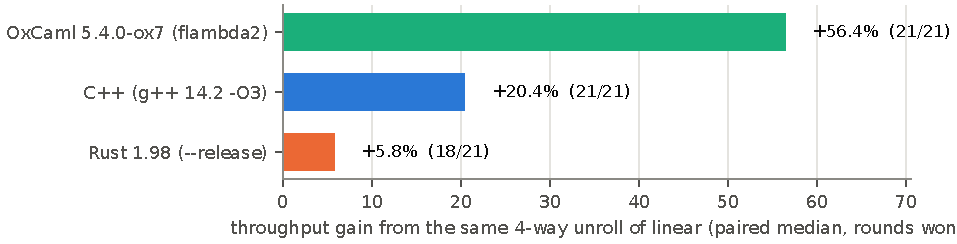
\includegraphics[width=0.78\textwidth]{fig_unroll}
  \caption{The same source change on three compilers (run W, paired median and
  rounds won).}
  \label{fig:unroll}
\end{figure}

\subsection{Two OCaml Compilers}
On the plain kernel flambda2 is $+41.2\%$ (21/21) faster
than the closure middle end ($+108.5\%$ (21/21) with
\code{-unsafe}); on the unrolled kernel it shrinks to
$+4.2\%$ (15/21). On the plain kernel the closure
compiler does not inline the inner loop's local function: it allocates a
closure per row and keeps the accumulator boxed, so each multiply--add costs
21 instructions and 16 bytes of allocation. flambda2 turns it into a loop with
the accumulator in a register (12 instructions, no allocation). The unrolled
kernel is already a loop, and there the two compilers are close.

\subsection{Where Stage I Ended}
OxCaml became $2.54\times$ faster than its first
version, and the gap to scalar C++ fell from $4.19\times$ to
$1.65\times$ ($1.78\times$ to vectorised C++).
Everything after this leaves the OCaml source alone.

\section{Stage II: Where the Remaining Time Goes}
\label{sec:stage2}

\subsection{Region Profiling}
\label{sec:regions}
flambda2 inlines the whole forward pass into one symbol, which a sampling
profiler cannot split, so I wrote a region profiler
(\code{tools/profile_regions.py}) that instruments the C++ and OCaml ports at
identical region boundaries with the time-stamp counter. The counters perturb
the compilers differently (scalar C++ lost 9.8\% throughput, OxCaml 5.2.0+ox
6.7\%), so each region's \emph{share} comes from the instrumented run and the
total from the uninstrumented binary. The regions cover 97--100\% of the
forward pass.

\begin{figure}[h]
  \centering
  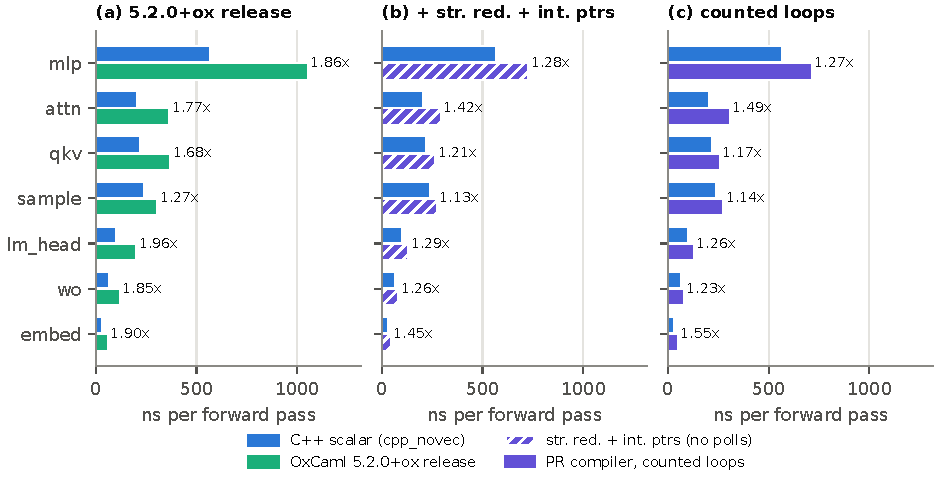
\includegraphics[width=\textwidth]{fig_regions}
  \caption{Nanoseconds per forward pass by region against scalar C++
  (1,431\,ns per token), separate region-profile run (7 rounds); labels give
  the OCaml/C++ ratio. (a) OxCaml 5.2.0+ox release, unrolled kernel:
  2,471\,ns ($1.73\times$). (b) Strength reduction and interior pointers, no
  polls (Section~\ref{sec:ip}): 1,815\,ns ($1.27\times$). (c) Counted loops,
  polls at loop exits (Section~\ref{sec:counted}): 1,810\,ns ($1.26\times$).}
  \label{fig:regions}
\end{figure}

No single region is pathological. The four regions dominated by \code{linear}
(\code{mlp}, \code{qkv}, \code{lm_head}, \code{wo}) run at similar ratios,
$1.69$--$1.95\times$ (C++ about 0.25\,ns per multiply--add, OxCaml about
0.47), and account for 75\% of the gap; \code{sample}, which spends much of
its time in the same C library \code{exp}, is closest ($1.27\times$). The
bottleneck is \code{linear}'s inner loop.

\subsection{The Gap Is Not SIMD}
The shipped C++ kernel contains 27 packed SSE2 instructions; OxCaml emits only
scalar arithmetic. Yet GCC's vectoriser is worth only
$+9.5\%$ (21/21) to C++, and scalar C++ is still
$1.65\times$ faster than OxCaml. The gap is scalar overhead around
the arithmetic.

\subsection{The Hot Loop, Instruction by Instruction}
\label{sec:hotloop}

\begin{lstlisting}[language=asmX,caption={OxCaml 5.2.0+ox, where this work began, unrolled kernel: 23 instructions per 4 MACs.},label=lst:ox-hot]
vmovsd -0x4(%rax,%rbp,4),%xmm4        # x.(i)
mov    %r9,%r10                       # rebuild b0 + i ...
add    %rbp,%r10                      # ... every iteration
vmulsd -0x8(%rbx,%r10,4),%xmm4,%xmm5  # d.(b0+i), load folded into the multiply
vaddsd %xmm5,%xmm3,%xmm3
mov    (%rsp),%r10                    # b1 was spilled: reload it
add    %rbp,%r10
vmulsd -0x8(%rbx,%r10,4),%xmm4,%xmm5
vaddsd %xmm5,%xmm2,%xmm2
# ... rows 2 and 3: the same mov / add / vmulsd / vaddsd ...
cmp    %r13,%rbp                      # exit test before the increment
je     .Lexit
add    $0x2,%rbp                      # i++ (tagged, step 2)
cmp    (%r14),%r15                    # GC safepoint poll
jbe    .Lgc
jmp    .Ltop                          # extra unconditional back edge
\end{lstlisting}

\begin{lstlisting}[language=asmX,caption={C++ with \texttt{-fno-tree-vectorize}: 15 instructions per 4 MACs.},label=lst:cpp-hot]
movsd  (%rcx,%rax), %xmm0     # x[i]
movsd  (%rdi,%rax), %xmm5     # w0[i]
mulsd  %xmm0, %xmm5
addsd  %xmm5, %xmm4
movsd  (%rsi,%rax), %xmm5     # w1[i]
mulsd  %xmm0, %xmm5
addsd  %xmm5, %xmm3
movsd  (%rdx,%rax), %xmm5     # w2[i]
mulsd  %xmm0, %xmm5
mulsd  (%r8,%rax), %xmm0      # w3[i]
addq   $8, %rax               # ONE offset advances all four rows
addsd  %xmm5, %xmm2
addsd  %xmm0, %xmm1
cmpq   %rax, %r9
jne    .L13
\end{lstlisting}

Both inner loops (Listings~\ref{lst:ox-hot} and~\ref{lst:cpp-hot}) do the same
8 floating-point operations; the 5.4.0-ox7 release emits the same loop
structure (21 instructions including the poll). The difference is integer
bookkeeping, with five sources:

\begin{enumerate}
  \item \textbf{No interior pointers} (8 instructions): OCaml rebuilds
        \code{b_k + i} for every row on every iteration, where C++ keeps four
        row pointers and one shared offset.
  \item \textbf{A register spill} (one of those 8 is a stack load): with
        \reg{r14} and \reg{r15} reserved and \reg{r11} unavailable across the
        poll, one row base lives on the stack.
  \item \textbf{The safepoint poll} (2 instructions), although the loop
        neither allocates nor calls.
  \item \textbf{Loop shape} (1 extra instruction): the poll block forces an
        unconditional \code{jmp}.
  \item \textbf{Tagging}, which costs nothing: scale-4 addressing absorbs it.
\end{enumerate}

Figure~\ref{fig:budget} summarises the budget and where the compiler work of
Sections~\ref{sec:sr}--\ref{sec:ip} takes the loop. The instruction ratio,
23/15 = $1.53\times$, is of the same size as the measured gap
($1.65\times$ on the release), but one counts the inner loop alone and the other
times the whole program, about a quarter of whose gap lies outside
\code{linear}.

\begin{figure}[h]
  \centering
  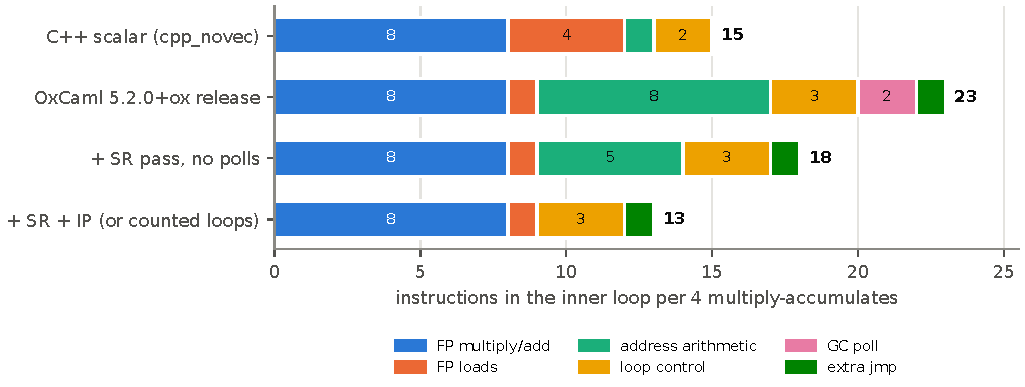
\includegraphics[width=0.9\textwidth]{fig_budget}
  \caption{Inner-loop instructions per four multiply--accumulates. The two
  lower rows are the passes of Sections~\ref{sec:sr} and~\ref{sec:ip} on a
  compiler configured without polls; with polls on, counted loops give the
  same 13-instruction loop.}
  \label{fig:budget}
\end{figure}

The first cause belongs to the language and its collector; the second to fourth
to the compiler.

\section{Stage III: The Safepoint Tax}
\label{sec:polls}

My guide suggested pricing the poll with two experiments that bracket its cost.

\subsection{Two Ways to Remove a Poll}
\begin{itemize}
  \item \textbf{NOP patch (lower bound).} \code{tools/nop_polls.py}
        overwrites every \ainl|cmp (%r14),%r15| plus \code{jbe} pair (a poll)
        in the linked binary with multi-byte NOPs, aborting unless every poll
        is gone and the count of similar-looking allocation checks is
        unchanged (in the first binary patched, 853 polls and 1,263 checks).
        The output stays bit-identical, and registers and layout are
        untouched.
  \item \textbf{Compiler flag (upper bound).} \code{-disable-poll-insertion}
        recompiles without polls, so the compiler can re-optimise around
        their absence.
\end{itemize}

Removing polls is correct for single-domain microgpt, not in general
(Section~\ref{sec:reality}).

\subsection{Results: What You Remove Is Not What You Pay}
\label{fig:polls}
On the release's plain kernel, which executes about four times as many
back-edge polls as the unrolled one, the NOP patch gains
$+1.1\%$ (14/21) and the flag
$+9.7\%$ (18/21). On the unrolled kernel
the NOP patch gains $+3.9\%$ (19/21)
(interquartile range $[+1.6, +6.7]\%$)
and the flag $+4.3\%$ (14/21).
Executing the poll costs a few percent at most; recompiling without polls can
be worth several times that. On the unrolled kernel the two are close because
5.4.0-ox7's poll-free build re-tags the index with an extra \code{lea} that
forces a spill: it is 12.5\%
slower than the same build on the previous release, 5.2.0+ox.

\subsection{The \texorpdfstring{\%r11}{r11} Exclusion}
\label{sec:r11}
On 5.2.0+ox, without polls \code{linear} shrinks from 102 to 91 instructions, its one
stack spill disappears, and register \reg{r11} goes from 0 uses to 8. The
backend declares \reg{r11} destroyed at every poll and allocation
(\code{destroyed_at_alloc_or_poll} in \code{backend/amd64/proc.ml}), so with a
poll in the loop the allocator spills a row base.

A binary patch that rewrote the two spill instructions into moves through
\reg{r11} (same instruction count, no spill) gained only $+0.3\%$ (7/11
rounds, a separate run): the slot is in L1 and off the critical floating-point
chain, so the spill is not where the poll's cost lies. The runtime does save
\reg{r11} in \code{SAVE_ALL_REGS}~\cite{ocaml_runtime}, and an OCaml core
developer told me the exclusion may be redundant in the non-PLT
configuration; settling it needs a test that forces the slow path with a
pointer in \reg{r11}.

What, then, makes the flag worth more than the poll it removes? On the
release it changes code layout, block structure and register allocation
together, and these experiments cannot separate them. On the patched compiler
most of the value of removing polls is in the optimisations their absence
\emph{permits} (Section~\ref{sec:reality}).

\paragraph{Configuration for the next stages.} Stages IV to VI develop the
passes on compilers built without poll insertion, to study the address
arithmetic with no poll in the loop; Stage VII measures them with polls on,
the configuration OxCaml is released with. The final measurement of each pass
(Table~\ref{tab:passes}) uses the pull-request compiler configured like the
release, with counted loops (Section~\ref{sec:counted}).

\section{Stage IV: Strength Reduction in the Compiler}
\label{sec:sr}

\subsection{The Missing Optimisation}
In the inner loop \code{b_k} is invariant and \code{i} grows by a constant, so
\code{b_k + i} is itself an induction variable that could be incremented per
iteration instead of rebuilt with a \code{mov} and an \code{add}: \emph{strength
reduction}~\cite{cocke1977strength}. A six-line reproducer shows that flambda2
does not do it:

\begin{lstlisting}[language=OCamlX,caption={Strength-reduction reproducer.},label=lst:sr-repro,numbers=none]
let f (d : float array) (x : float array) b0 cols =
  let a = ref 0.0 in
  for i = 0 to cols - 1 do a := !a +. (d.(b0 + i) *. x.(i)) done; !a
\end{lstlisting}

\begin{lstlisting}[language=asmX,caption={Its inner loop under OxCaml 5.2.0+ox, \texttt{-O3 -unsafe}.},label=lst:sr-asm]
.L109: movq    %rdi, %rcx                # reload the invariant b0
       addq    %rdx, %rcx                # recompute b0 + i, every iteration
       vmovsd  -8(%rax,%rcx,4), %xmm1    # d.(b0+i): two extra instructions
       vmulsd  -4(%rbx,%rdx,4), %xmm1, %xmm1   # x.(i): none, i is the counter
       vaddsd  %xmm1, %xmm0, %xmm0
       cmpq    %rsi, %rdx
       je      .L118
       addq    $2, %rdx                  # i++ (tagged)
       cmpq    (%r14), %r15              # poll
       jbe     .L126
       jmp     .L109
\end{lstlisting}

In the same loop \code{x.(i)} costs no extra instructions because \code{i} is
the counter, while \code{d.(b0 + i)} costs two, with or without bounds checks.

Is this cost imposed by the language or by the compiler? Writing the C++
kernel in OCaml's index form, \code{d[b0 + i]}, separates the two: if the
index form were inherently costly, it would carry the same extra
instructions; if the cost lies in the compiler, GCC would remove them. It
compiles to the same 15-instruction loop as the pointer version and runs
equally fast (a separate 21-round run): GCC strength-reduces the index. The
language forces OCaml into the index form, but only its compiler leaves it
unoptimised, so a compiler pass is the right fix.

\subsection{By Hand First}
Carrying four running indices \code{j0..j3} in the source (build switch
\code{MG_SR=1}) removed the eight rebuild instructions and the spill (on
5.2.0+ox the loop shrank from 23 to 21 instructions), gaining
$+10.3\%$ (21/21) on the OxCaml release.

On stock OCaml 5.3.0 the same edit gave
$+12.3\%$ (20/21). But a source-level workaround must be
repeated by hand in every loop and makes the source harder to read.

\subsection{Confirming the Gap in the Compiler Source}
Neither flambda2's catalogue of optimisations nor any of 29,035 commits
mentions loops, induction or strength; there is no loop-invariant code motion,
value numbering or unrolling. My guide
suggested contacting the OCaml maintainers and first opening the change as a
pull request to my own fork.

\subsection{A Strength-Reduction Pass over Cmm}
\label{sec:sr-pass}
I implemented the pass on Cmm rather than in flambda2
(Figure~\ref{fig:pipeline}). Cmm has no assignment, so ``bound outside the
loop'' \emph{is} the invariance analysis.

\begin{figure}[h]
  \centering
  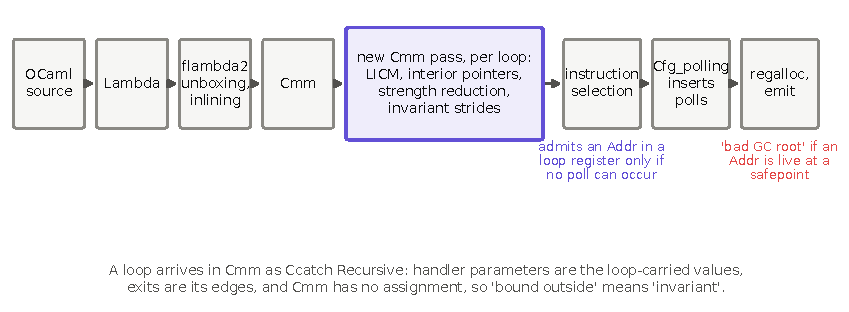
\includegraphics[width=\textwidth]{diag_pipeline}
  \caption{The new pass in the OxCaml backend; the checks on the right make
  interior pointers safe (Section~\ref{sec:ip}).}
  \label{fig:pipeline}
\end{figure}

The pass finds a counter \code{c} that every back edge steps by a constant
$n$, collects variables affine in it ($m\cdot c + k$), and rewrites every sum
\code{inv + idx}, with \code{idx} affine and \code{inv} an integer bound
outside the loop, into a loop parameter starting at \code{inv + (m*c0 + k)}
and stepping by $m\cdot n$:

\begin{lstlisting}[language=CmmX,caption={The transformation in pseudo-Cmm (tagged index $i = 2c + 1$).},label=lst:sr-cmm]
; before
(catch rec (loop c a0 a1 a2 a3)
   ... (load float64 (+a (+a d (<< (+ b1 i) 2)) -8)) ...
   (exit loop (+ c 1) ...))
; after: b1 + i is carried as sr1
(catch rec (loop c a0 a1 a2 a3 sr1)
   ... (load float64 (+a (+a d (<< sr1 2)) -8)) ...
   (exit loop (+ c 1) ... (+ sr1 2)))
with entry (exit loop 0 0. 0. 0. 0. (+ b1 1))
\end{lstlisting}

Both operands must be integers (a carried value is live across the back-edge
poll, so it must never be a pointer), and variables bound more than once are
ignored; wrapping addition is associative, so overflow behaviour is
unchanged. Three cost rules decide whether a rewrite pays:

\begin{itemize}
  \item \textbf{Register neutrality.} The invariant must have \emph{no other
        use} in the loop, so it dies at entry.
  \item \textbf{Only sums that must be materialised.} OCaml's tagged indices
        reach Cmm as \code{(base + i) - 1}, which x86 forms with one
        \code{lea}; carrying such a sum only adds an \code{add} and a live
        register. Skipping these sums makes nx-oxcaml's element-wise kernels
        1.10--1.14$\times$ faster under default flags, the passes-off speed
        (a separate 15-round run).
  \item \textbf{At most eight carried values.} Without this cap a loop with 24
        such sums ran 1.65$\times$ slower than with the pass off; with it, the
        loop runs at the passes-off speed.
\end{itemize}

The pass sits behind \code{-[no-]cmm-strength-reduction}; with the flag off
the code is byte-identical.

\subsection{Results}
\begin{itemize}
  \item \textbf{Correctness.} 17 hand-written edge cases (counting down,
        overflow, exceptions, forced major GCs) and 30 random programs match
        the pass off; Section~\ref{sec:counted} gives the test suite.
  \item \textbf{Speed on unmodified source.} $+10.5\%$ (19/21) on the
        final compiler with counted loops (Table~\ref{tab:passes}), and
        $+13.3\%$ (21/21) on the compilers built without polls, close to
        the hand edit's $+10.3\%$.
  \item \textbf{Code.} The pass leaves one re-tag the hand edit does not,
        \ainl|leaq 1(%r10,%r10)|, from the translation to Cmm; interior
        pointers (Section~\ref{sec:ip}) remove it.
\end{itemize}

The pass does not cover non-constant strides (Section~\ref{sec:ivs}) or
invariant expressions that flambda2 has inlined into an address, which
explains the crypto-study result (Section~\ref{sec:crypto}).

\section{Stage V: Interior Pointers}
\label{sec:ip}

\subsection{The Idea}
After strength reduction the loop still increments four indices; C++
increments one offset shared by four row pointers. My guide proposed a way to
close the difference: \emph{show that the hot loop does not
allocate, and if GC polls are disabled, interior pointers are allowed inside
that block.} A loop with no allocation, call or poll contains no safepoint, so
a derived pointer created before it and dead after it is never seen by the
collector.

\subsection{Permission versus Transformation}
Pointers into OCaml's Bigarrays, which live outside the heap, are already
legal: the \emph{permission} is granted. Yet a Bigarray kernel compiled to 19
instructions per 4 MACs instead of 18, reloading the data pointer every
iteration: the \emph{transformation} was missing regardless. I therefore made
the compiler form interior pointers into ordinary OCaml arrays.

Polls are inserted long after Cmm, but a loop that neither allocates nor calls
gets a back-edge poll unless poll insertion is disabled, so the condition
reduces to two checks available on Cmm: the loop body is \emph{GC-free}, and
polls are disabled. Counted loops (Section~\ref{sec:counted}) later replace
the second check.

\subsection{Design}
\label{sec:ip-design}
The pass extends the strength-reduction pass. For a recursive \code{catch}:

\begin{enumerate}
  \item \textbf{GC-freedom.} \code{is_gc_free} rejects a loop body containing
        any call, allocation, poll, probe, region operation, atomic, or integer
        division (whose zero-divisor path is a call). The match over Cmm
        operations is exhaustive, so a new operation becomes a compile error.
        Raising is allowed: the raise records an empty live set.
  \item \textbf{Re-association and hoisting.} An access \code{a.(b + i)}
        reaches Cmm as \code{(+a (+a a (<< (+ b i) 2)) -8)} with
        $i = m\cdot c + k$. Shifts distribute over wrapping addition, so this
        equals \code{(+a (+a (+a a (<< b 2)) (<< c 3)) -4)}; \code{a + 4b} is
        bound once before the loop as an \code{Addr} and the access becomes
        \code{disp(base, counter, 8)}. Four rows share one index register and
        one increment, and the untagged counter removes the re-tag of
        Section~\ref{sec:sr-pass}.
  \item \textbf{Safety net.} If the analysis were wrong, an \code{Addr} live at
        a safepoint would stop compilation with \code{bad GC root}, never
        corrupt the heap.
\end{enumerate}

Interior pointers run before strength reduction on each loop and subsume it on
the accesses they rewrite; with \code{-no-cmm-interior-pointers} the output is
byte-identical to the strength-reduction compiler.

\subsection{Verification}
Of three small loops (clean, calling a closure, allocating) only the clean
one was transformed (10 to 6 instructions). With \code{is_gc_free} stubbed to
return \code{true}, the other two failed with
\ainl|Fatal error: bad GC root ip_base:A/46[%rdi]|: the backend check catches
any derived pointer live at a safepoint. It does not check the address
arithmetic itself or the termination proof of Section~\ref{sec:counted}; the
test suite, adversarial loops and GC stress tests cover those.

\subsection{Results}
\begin{lstlisting}[language=asmX,caption={Inner loop with strength reduction and interior pointers (no polls): 13 instructions per 4 MACs. The final compiler with counted loops emits the same loop with polls on.},label=lst:ip-loop]
# preheader: four hoisted row bases (Addr), formed once
leaq    (%rbx,%r13,4), %r13
leaq    (%rbx,%r12,4), %r12
leaq    (%rbx,%r9,4),  %r9
leaq    (%rbx,%r8,4),  %r8
.L168:
vmovsd  (%rax,%r11,8), %xmm4             # x.(i), untagged counter
vmulsd  -4(%r8,%r11,8), %xmm4, %xmm5     # row 0: base + shared index
vaddsd  %xmm5, %xmm3, %xmm3
vmulsd  -4(%r9,%r11,8), %xmm4, %xmm5     # row 1: same index register
vaddsd  %xmm5, %xmm2, %xmm2
vmulsd  -4(%r12,%r11,8), %xmm4, %xmm5
vaddsd  %xmm5, %xmm1, %xmm1
vmulsd  -4(%r13,%r11,8), %xmm4, %xmm4
vaddsd  %xmm4, %xmm0, %xmm0
incq    %r11                             # ONE increment for all four rows
cmpq    %rbp, %r11
jg      .Lexit
jmp     .L168
\end{lstlisting}

The hot block went from 18 to 13 instructions (Listing~\ref{lst:ip-loop}).
On the final compiler with counted loops, interior pointers are worth
$+13.9\%$ (20/21) on top of strength reduction, leaving OxCaml
$1.26\times$ behind scalar C++ (on the compilers built without polls,
$+12.8\%$ (21/21)), with identical output. The loop
executes fewer instructions per MAC than C++'s (13 against 15), yet the
\code{linear} regions still run $1.21$--$1.29\times$ slower
(Figure~\ref{fig:regions}(b)): instruction count had stopped being the
explanation. Interior pointers form only in loops without polls; on the
compilers of this stage that is every GC-free loop (Section~\ref{sec:reality}
measures the release configuration).

\section{Stage VI: The Outer Loop and a Register-Bound Kernel}
\label{sec:stage6}

\subsection{Invariant-Stride Induction Variables}
\label{sec:ivs}
With the inner loops nearly identical to C++, the difference moved to the
\emph{row-group} loop. GCC advances four row pointers with four \code{addq}s
per group; OxCaml rebuilt them with an \code{imulq} and eight \code{leaq}s.
The row base \code{o * cols} steps by \code{4 * cols}, an invariant but not
constant stride, which strength reduction declines:

\begin{lstlisting}[language=CmmX,caption={The row bases in Cmm (tagged arithmetic).},label=lst:rowbases,numbers=none]
b0 = (+ (* (+ o -1) (>>s cols 1)) 1)    ; a product with a runtime stride
b1 = (+ (+ b0 cols) -1)
b2 = (+ (+ b0 (<< cols 1)) -2)
b3 = (+ (+ b0 (* cols 3)) -3)
\end{lstlisting}

The invariant-stride pass generalises the affine model to
\code{pointer + (stride * counter + offset)}, with stride and offset
\emph{expressions} over variables bound outside the loop. The stride is
computed once and each back edge becomes one pointer addition; since the pass
carries the four interior \emph{pointers}, the \code{imulq}/\code{leaq} chain
becomes dead. Instruction selection now allows an \code{Addr} in a
loop-carried register under the pass's condition; the \code{bad GC root}
check still applies. The preamble fell from 25 to 13 instructions, the shape
GCC emits. Carrying the indices
instead (\code{-no-cmm-carried-pointers}) keeps nine values live instead of
four and spills in the hot loop: on the compilers built without polls,
carrying pointers is $+31.3\%$ (21/21) faster, and the pass is
worth $+4.2\%$ (15/21) over interior pointers alone.

\subsection{Loop-Invariant Code Motion: A Designed Null Result}
The inner loop's trip count, \code{(cols - 2) >>s 1}, is recomputed for every
row group although it is invariant; flambda2 has no loop-invariant code
motion~\cite{aho2006dragon}, so the LICM pass hoists pure integer
\code{let}-bindings out of GC-free loops. Hoisting unconditionally made the
allocator spill a value inside the inner loop (visible in the assembly; the
measured $-1.1\%$, in a separate 15-round run, is within the noise): a hoist
is free only if its operands die, and \code{cols} does not. LICM therefore
uses strength reduction's register-neutrality condition and, on microgpt,
declines as designed: \code{pr_c_ivs} and \code{pr_counted} compile to the
same code, and the measured difference, $+0.5\%$ (13/21), shows the
run's resolution. Whether it hoists depends on the loop, not on this
benchmark.

\paragraph{Observation: spills track the result.} Every change that made the
allocator spill inside the inner loop lost (carried indices, unconditional
hoisting); every change that removed a live value or a spill won. Not every
spill is costly: an eight-row kernel (Section~\ref{sec:simd-why}) spills four
values per iteration yet runs as fast as the four-row kernel, because its L1
reloads, spread over eight multiply--adds, leave slightly fewer instructions
per multiply--add (about 3.1 against 3.25). A spill hurts when it adds work to
every multiply--add.

\subsection{The Ladder}
Table~\ref{tab:passes} gives each pass's contribution on the pull-request
compiler configured like the release. Counted loops (Section~\ref{sec:counted})
come first, so that polls sit at loop exits and every pass can act; source and
output are identical in every row.

\begin{table}[h]
  \centering
  \small
  \begin{tabularx}{\textwidth}{@{}lXrr@{}}
    \toprule
    step & what it does & paired gain (rounds) & gap \\
    \midrule
    passes off (\code{pr_off}) & polls on every back edge & & $1.69\times$ \\
    + counted loops & polls move to loop exits; nothing else changes & $+3.5\%$ (16/21) & $1.59\times$ \\
    + strength reduction & carries \code{base + i} as a loop parameter & $+10.5\%$ (19/21) & $1.46\times$ \\
    + interior pointers & one hoisted \code{Addr} per row, one shared index & $+13.9\%$ (20/21) & $1.26\times$ \\
    + invariant strides & carries the row pointers across the row loop & $-0.8\%$ (9/21) & $1.31\times$ \\
    + LICM (\code{pr_counted}) & declines here, by design (identical code) & $+0.5\%$ (13/21) & $1.29\times$ \\
    \midrule
    all, from passes off & & \textbf{$+30.2\%$} (21/21) & \\
    \bottomrule
  \end{tabularx}
  \caption{The pass ladder (pull-request compiler, unchanged source, run W);
  gap to scalar C++ in the last column.}
  \label{tab:passes}
\end{table}

Counted loops alone only remove polls; strength reduction and interior
pointers carry the gain. Invariant strides add nothing measurable here: with
counted loops, interior pointers already remove this kernel's row-group
arithmetic. With polls kept on every back edge, the four passes give only
$+10.2\%$ (21/21) (Section~\ref{sec:reality}).

\subsection{Where Is the Rest of the Gap?}
\label{sec:residual}
With invariant strides the regions dominated by \code{linear} run at
$1.15$--$1.25\times$ of scalar C++ and attention, at $1.42\times$, is the
worst; with counted loops the picture is the same ($1.17$--$1.27\times$,
attention $1.49\times$; Figure~\ref{fig:regions}). In isolated calls
(Table~\ref{tab:shapes}, left), $16\times64$, with four times as many columns
per row, has a larger gap than $64\times16$ with equal work, so part of the
gap lives in the inner loop body.

\begin{table}[h]
  \centering
  \small
  \begin{tabular}{@{}lrrr@{\hspace{3em}}lr@{}}
    \toprule
    shape (rows $\times$ cols) & C++ ns & OxCaml ns & ratio & hand-written loop & ticks/iter \\
    \midrule
    $64\times16$ (fc1)      & 228.5 & 240.9 & $1.05\times$ & C++ shape & 2.875 \\
    $16\times16$ (q, k, v, o) & 57.4 & 62.0 & $1.08\times$ & OxCaml shape & 3.305 \\
    $16\times64$ (fc2)      & 209.5 & 250.0 & $1.19\times$ & \quad rotated, one branch & 3.301 \\
    $27\times16$ (lm\_head) & 89.0 & 111.6 & $1.25\times$ & \quad loads not folded & 3.301 \\
    $28\times16$ (no remainder) & 88.4 & 105.0 & $1.19\times$ & \quad scale 1 instead of 8 & 3.309 \\
    \bottomrule
  \end{tabular}
  \caption{Separate micro-benchmarks. Left: isolated \texttt{linear} calls,
  scalar C++ against the invariant-strides compiler. Right: hand-written 4-MAC
  loops, in time-stamp-counter ticks per iteration (3.0\,GHz counter, core at
  about 4.4\,GHz: one tick is about 1.46 core cycles).}
  \label{tab:shapes}
\end{table}

\paragraph{Loop structure.} Hand-written assembly versions of both loop shapes,
varied one difference at a time (Table~\ref{tab:shapes}, right), showed that
rotating the loop, un-folding the loads and changing the addressing scale are
each worth nothing. Only the encoding (two-operand SSE in C++, three-operand
VEX in OxCaml) moved the result, and not cleanly: run alone, the SSE loop
slowed from 2.875 to 3.675 ticks, an SSE/AVX transition effect. A cleaner
test: if SSE favoured C++, building C++ with VEX (\code{-mavx}) should slow it
towards OxCaml. In run W that build is $-5.9\%$ (2/21) against
the SSE build, so the SSE baseline is the harder one to match, not a
flattering one.

\paragraph{A model of the core.} Why is a loop with fewer instructions than
C++'s slower? A loop can be limited by instruction issue, by its execution
ports, or by chains of dependent instructions; only the first depends directly
on instruction count. \code{llvm-mca} with its Alder Lake description (the closest
available model of this machine's Meteor Lake performance cores) predicts which
limit applies
(Table~\ref{tab:mca}; a floating-point addition takes 2 cycles and a
multiplication 3). It puts the patched 13-instruction loop level with C++'s
15: both push the same eight floating-point operations through the same two
ports, at least three cycles per iteration, so, in the model, removing integer
instructions cannot make it faster than C++'s. The 5.2.0+ox loop's 23
instructions exceed what the core can issue in three cycles, which is why
removing instructions paid off until the loop reached C++'s size.

\begin{table}[h]
  \centering
  \small
  \begin{tabular}{@{}lrrrl@{}}
    \toprule
    inner loop & instructions & predicted & measured & predicted bound \\
    \midrule
    C++ scalar (\code{cpp_novec}) & 15 & 3.02 & 3.22 & floating-point ports \\
    OxCaml, counted loops (\code{pr_counted}) & 13 & 3.02 & 3.66 & floating-point ports \\
    OxCaml, SSE2 kernel, no polls & 16 & 3.02 & 3.46 & shuffle port \\
    OxCaml 5.2.0+ox release & 23 & 4.02 & 5.84 & instruction issue \\
    \bottomrule
  \end{tabular}
  \caption{Core cycles per 4-MAC iteration: predicted by \code{llvm-mca}, and
  measured with each loop copied at its original alignment into a timing
  harness (a separate measurement, 256 columns).}
  \label{tab:mca}
\end{table}

Measured alone, the patched loop is about 14\% slower than C++'s, where the
model predicts no difference; the cause is not identified here. This bounds
the rest of the gap: if the inner loop were the whole story, the program would
be at most about 14\% slower than C++; it is $1.29\times$ behind, so
by this estimate roughly half of the remaining gap lies outside the inner
loop, in the
row-group setup (once per four rows of only 16 columns) and in the other
regions, attention above all.

\paragraph{Attention.} The attention loops call \code{linear} and
\code{softmax}, so the pointer passes do not apply. Swapping the value
gather's loop nest to do four MACs per iteration over contiguous memory took
OxCaml's attention block from 395 to 246\,ns in an isolated test, level with
unchanged C++ (248\,ns), which would gain too.

\section{Stage VII: Measuring With Safepoints On}
\label{sec:reality}

\subsection{Two Compiler Configurations}
Whether the compiler inserts safepoint polls is a configure option fixed when
it is built. The compilers of Sections~\ref{sec:sr} to~\ref{sec:stage6} were
built with \code{--enable-flambda2} alone, which inserts no polls. The release
also passes \code{--enable-poll-insertion} (Listing~\ref{lst:config}); this
stage measures the passes in that configuration.

\begin{lstlisting}[language=plaintext,caption={Configure options of the compilers of Stages IV--VI (top) and of the opam OxCaml release (bottom).},label=lst:config,numbers=none]
# compilers of Stages IV-VI
--enable-flambda2                      -> POLL_INSERTION=false

# opam release recipe, oxcaml-compiler 5.4.0-ox7
--enable-middle-end=flambda2 --enable-runtime5 --enable-stack-checks
--enable-poll-insertion --enable-multidomain
\end{lstlisting}

\subsection{What the Passes Are Worth With Safepoints}
\label{tab:pollladder}
On the pull-request compiler with the release options, four builds (passes
off and on, each with and without polls) produce identical output. Without
polls the
passes are worth $+28.9\%$ (21/21), as on the compilers built
without polls, but with polls on every back edge only
$+10.2\%$ (21/21), reaching $1.51\times$ behind scalar C++. Removing polls is
worth $+3.1\%$ with the passes off but $+18.2\%$
with them on. A pointer into an
array cannot be kept across a poll, so with a poll on every back edge interior
and carried pointers cannot form, and only strength reduction and invariant
strides survive, in their index form: most of the value of removing polls is
in the optimisations they block. With the flag, the pull-request compiler
matches the compilers built without polls ($-0.9\%$,
9/21 rounds). On the release, annotating functions with
\code{[@poll error]} is no alternative: it rejects any function containing a
loop that needs a poll.

\subsection{Why Polls Cannot Simply Be Turned Off}
Removing polls is safe only if no domain ever waits for another inside a
loop. nx-oxcaml, a numerical library that runs its kernels on a pool of
domains, ends each parallel operation with a spin-wait
(Listing~\ref{lst:spin}).

\begin{lstlisting}[language=OCamlX,caption={nx-oxcaml's spin-wait (\texttt{lib/parallel.ml}). Without a poll on its back edge, the main domain never reaches a safepoint.},label=lst:spin,numbers=none]
while Atomic.get pool.completed < pool.num_workers do
  Domain.cpu_relax ()
done
\end{lstlisting}

If a worker needs a stop-the-world collection while the main domain spins
here, each waits for the other forever: built without polls, the nx benchmark
hangs. Whether polls can be removed is a property of the whole program, so a
library cannot choose it for its users.

\subsection{The Passes on nx-oxcaml}
\label{sec:nx-first}
I built nx-oxcaml~\cite{nx_oxcaml} with the patched compiler and ran its
benchmark of 19 operations at three sizes in both configurations. With polls
the passes fired in about 40 modules, but no operation group changed by more
than $\pm1.5\%$ over 13 rounds: only the index forms can fire, nx's scalar
kernels already carry their indices by hand, and the analysis did not yet
recognise nx's SIMD loops (Section~\ref{sec:counted}).

Without polls, interior pointers changed the machine code of 30 of 58
modules. To test whether that static diff predicts the gains, 78 benchmark
cases were grouped by how many instructions interior pointers removed from
each kernel (Figure~\ref{fig:nxpart}). The control, cases with identical
code, moved by $-0.24\%$; cases that lost 30--46 instructions were $+22.4\%$
faster (median) and up to $+32\%$: scalar loops indexing three or more arrays
off one counter, for which nx has no SIMD path. Interior pointers are thus
worth a great deal in a real library, but only in a configuration that can
deadlock it.

\begin{figure}[h]
  \centering
  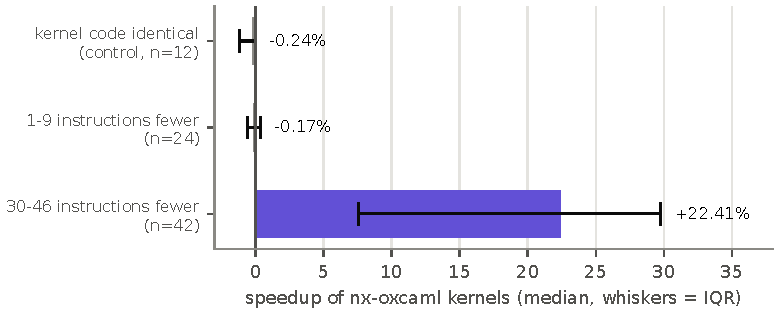
\includegraphics[width=0.66\textwidth]{fig_nx_partition}
  \caption{Speed-up from interior pointers on nx-oxcaml without safepoints (78
  cases, 21 interleaved rounds), grouped by instructions removed per kernel;
  medians with interquartile-range whiskers.}
  \label{fig:nxpart}
\end{figure}

\subsection{Bounding the Wait: Strip Mining}
Strip mining, a polled outer loop around poll-free strips of a fixed number of
iterations, keeps a fixed bound on the time to the next safepoint. Each strip
is itself a counted loop, so pointers can form inside it and are recomputed
after each outer poll; this is how HotSpot's C2 bounds the
wait~\cite{jdk_stripmining}. I did not build it. Counted loops
(Section~\ref{sec:counted}) poll at loop exits instead, with an optional trip
cap as a coarser bound; strip mining is the natural next step for bounding
latency.

\section{Stage VIII: Moving Polls to Loop Exits --- Counted Loops}
\label{sec:counted}

Two limitations remained: the analysis missed nx's SIMD loops, and the poll
on every back edge rules out interior and carried pointers
(Section~\ref{sec:reality}). A generalised analysis addresses the first,
counted loops the second.

\subsection{Generalising the Address Analysis}
Two patterns hid nx's SIMD loops from the analysis. First, SIMD operations
such as \code{caml_sse2_float64x2_add} reach Cmm as external calls, which
\code{is_gc_free} treated as safepoints; they are \code{[@@noalloc]} builtins
expanded inline, so the check now ignores them. Second, a 128-bit load from
an unboxed float array untags the index with a right shift before scaling,
\code{(+a a (<< (>>s idx 1) 3))}. Writing each index as $y + 2q$, with $q$
a constant, all accesses to one array at the same $y$ should share one
pointer. The identity $(y + 2q) \gg_s 1 = (y \gg_s 1) + q$ holds for
integers but not for 64-bit words: when $y + 2q$ wraps, the two sides differ
by $2^{63}$. The whole byte address is exact nonetheless. With $a$, $y$ and
$q$ 64-bit words read as signed integers and an element of $2^s$ bytes,
$1 \le s \le 3$, the machine computes $w = y + 2q - 2^{64}t$ for some integer
$t$, and $w \gg_s 1 = \lfloor w/2 \rfloor = \lfloor y/2 \rfloor + q -
2^{63}t$ because $2q$ and $2^{64}t$ are even. Scaling by $2^s$ makes the error
$2^{63+s}t$ a multiple of $2^{64}$, so
\[
  a + \bigl(((y + 2q) \gg_s 1) \ll s\bigr) \equiv
  a + \bigl((y \gg_s 1) \ll s\bigr) + (q \ll s) \pmod{2^{64}}
\]
for every $y$ and $q$. The same argument with $2q$ replaced by the counter's
even step $m\cdot n$ shows that a carried pointer advanced by
$(m n / 2) \ll s$ per iteration equals the original address on every
iteration, whatever wraps. The pass also accepts $s = 0$, where the error does
not vanish; there it relies on the original access being in bounds, which an
index whose sum wraps cannot be. With both rules, nx's 8-wide SIMD addition loop shrinks from 52 to 22 instructions
(Listing~\ref{lst:nx-simd}).

\begin{lstlisting}[language=asmX,caption={nx-oxcaml \texttt{add\_float64}, 8-wide SIMD loop, before (24 lea/sar pairs, back-edge poll) and after (one carried pointer per array).},label=lst:nx-simd]
# before (52 instructions, excerpt)
leaq    4(%r10),%rbp
sarq    $1,%rbp                    # untag the index ...
vmovupd (%rsi,%rbp,8),%xmm0        # ... then scale it, for every access
...
addq    $16,%rcx ; addq $16,%rdi ; addq $16,%rax ; addq $16,%rbx
cmpq    (%r14),%r15                # poll on the back edge
jbe     .L393
# after (22 instructions with counted loops)
vmovupd 8(%rax),%xmm0              # constant offsets from carried pointers
vmovupd 8(%r11),%xmm1
vaddpd  %xmm1,%xmm0,%xmm0
vmovupd %xmm0,8(%r10)
...
addq    $64,%r11 ; addq $64,%rax ; addq $64,%r10
\end{lstlisting}

\subsection{Counted Loops}
A loop that is guaranteed to finish and cannot reach the collector can poll
once \emph{after} the loop instead of on every back edge, as a
\code{[@@noalloc]} C call does. No domain is left in an unsafe state, but a
counted loop's time to the next safepoint is its running time. Termination is
essential: a poll-free spin-wait (Listing~\ref{lst:spin}) would stall every
other domain for ever. Under
\code{-cmm-counted-loops}, a GC-free loop with no polled loop inside loses its
back-edge poll if termination is proved, and polls on every exit instead
(Figure~\ref{fig:counted}). Interior and carried pointers are then legal
inside it, since exit values are computed \emph{before} the exit poll. A loop
whose only GC point is on the way out, such as boxing a result, also
qualifies.

A separate two-domain test (three repetitions per case) measures this cost.
One domain repeatedly runs a counted dot product over $N$ floats while a
second allocates and records its longest pause, each minor collection waiting
for the first domain's next safepoint. If the wait is one run of the loop,
the pause should grow with $N$, and it does: with back-edge
polls it stays within the host's jitter (1--4\,ms); with counted loops it
tracks the loop's running time, about 10\,ms for $N = 10^7$ (one run takes
8\,ms) and 74--85\,ms for $N = 10^8$ (70--73\,ms).

\paragraph{A trip cap.} \code{-cmm-counted-loops-max-trips N} (off by
default) keeps the polled copy for any loop that may run more than $N$
iterations. In a later run of the same test with the final passes and a cap
of $10^6$, the worst pause fell from 57--61\,ms to 0.5--1.1\,ms at $N = 10^8$
and from 546--592\,ms to 0.6--2.1\,ms at $N = 10^9$, against 0.4--1.2\,ms
without the pull request. With that cap microgpt runs at $0.848\times$ the
uncapped speed: the cap check reads the loop's start value, so it cannot be
lifted out of an inner loop, and the outer loops of nests lose counted status.

\begin{figure}[h]
  \centering
  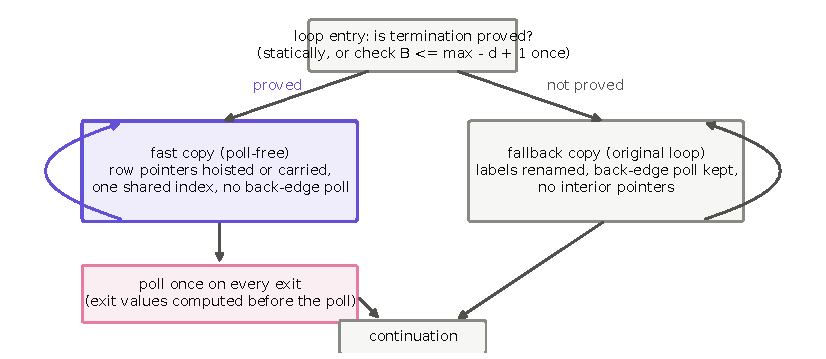
\includegraphics[width=0.86\textwidth]{diag_counted}
  \caption{A counted loop. If termination is not decided at compile time, the
  loop is compiled twice and a single check on entry selects the poll-free
  copy or the original, polled copy.}
  \label{fig:counted}
\end{figure}

\subsection{An Exact Termination Proof}
Loops can wrap around (\code{while i < n do i := i + 16} never ends if
\code{n} is within 15 of \code{max_int}), so the rule is exact in 64-bit
wrapping arithmetic. A loop qualifies when a counter $c$ is stepped by the
same non-zero constant $n$ on every back edge and a test $x \mathrel{R} B$,
with $x = m\cdot c + k$, $m \ne 0$ and $B$ invariant, dominates every back
edge; $x$ then changes by exactly $d = m\cdot n$ per iteration, and the loop
ends under the preconditions of Table~\ref{tab:termination}. Cmm already
holds OCaml integers as tagged machine words, so $c$, $m$, $n$, $k$ and $B$
are machine-word quantities and tagging needs no separate case. The analysis
accepts only $|m|, |d| \le 2^{20}$, which makes $d$ exact and non-zero for
any step below $2^{43}$; a loop whose test does not move ($d = 0$) is never
counted.

\begin{table}[h]
  \centering
  \small
  \begin{tabular}{@{}ll@{}}
    \toprule
    loop continues while & proved to terminate when \\
    \midrule
    $x < B$, $d > 0$ & $B \le \textit{max} - d + 1$ \\
    $x \le B$, $d > 0$ & $B \le \textit{max} - d$ \\
    $x > B$, $d < 0$ & $B \ge \textit{min} - d - 1$ \\
    $x \ge B$, $d < 0$ & $B \ge \textit{min} - d$ \\
    $x \ne B$, $|d| = 2^k$ & $x_0 \le B$ and $(B - x_0) \bmod |d| = 0$ (mirrored for $d < 0$) \\
    $x = B$, $d \ne 0$ & always (the test fails by the second iteration) \\
    anything else & never \\
    \bottomrule
  \end{tabular}
  \caption{Termination preconditions. For example, $i \ne n$ stepping by 2
  never ends if $n - i$ is odd.}
  \label{tab:termination}
\end{table}

A small interval analysis decides the precondition at compile time where it
can (microgpt's trip count \code{(cols - 2) >> 1} can never approach
\code{max_int}); otherwise one check on entry selects between two copies of
the loop. Checks that depend only on outer-loop invariants are lifted
outward, making a nest one poll-free region behind one check; nests inside
loops that still poll get no exit polls, since the enclosing poll bounds the
time to the next safepoint. A size budget limits the fallback copies: a
12-deep nest's code shrinks from 5,712 to 2,912 bytes, and microgpt is
unchanged. \code{-dcounted-loops} prints each loop's decision and reason.

\paragraph{Why it is safe.} A derived pointer is never live across a GC
point, because interior and carried pointers form only in loops with no
allocation, call or poll. The backend's \code{bad GC root} check rejects any
violation at compile time. Other domains' stop-the-world sections need this
domain to poll, which it does at loop exit. The collector is not idle
meanwhile: other domains may mark and sweep the major heap concurrently.
Marking never moves an object, and sweeping frees only objects that were
unreachable when the major cycle began, which the loop's arrays were not.
What moves objects, minor collections and compaction, is stop-the-world in
OCaml~5 and so must wait until this domain reaches a safepoint; no object a
derived pointer points into can move while the loop runs. The termination proof is exact in 64-bit wrapping
arithmetic, so every counted loop reaches its exit poll. These are two
guarantees: the collector never sees a derived pointer, and every domain
eventually polls. A third, a bound on how long another domain waits, does not
follow from termination; that is the latency measured above, and the trip cap
bounds iterations without a poll, not their running time.

\subsection{Unchecked Loops}
My guide asked for a variant without the termination proof.
\code{-cmm-unchecked-loops} gives every GC-free loop the optimisation and also
drops back-edge polls in loops that contain calls; on microgpt it makes 78 of
the 86 loops poll-free (the other 8 contain an exception handler). Apparent
spin-waits (loops containing \code{Domain.cpu_relax} or an atomic) keep their
poll; loops with a tail call or an exception handler get no exit poll; and the
runtime's never-polled method-dispatch helpers are skipped in both modes. A
loop waiting on a plain mutable field loses its poll, so the mode stays opt-in
(Section~\ref{sec:liveness}).

\subsection{Giving Up Liveness}
\label{sec:liveness}
Three builds remove polls from loops without a termination proof
(Table~\ref{tab:liveness}). Their output is correct, but their loops can no
longer be preempted, and a loop that waits on another domain or a signal may
never terminate. None beats counted loops by more than about the run's
resolution: once the pointer passes can act, the remaining polls cost little,
and on the release, removing polls without the passes gains little.

\begin{table}[h]
  \centering
  \small
  \begin{tabular}{@{}llrrr@{}}
    \toprule
    build & polls removed by & tokens/s & vs scalar C++ & vs \code{pr_counted} \\
    \midrule
    \code{pr_unchecked} & \code{-cmm-unchecked-loops} & 585,497 & $1.22\times$ & $+3.3\%$ (17/21) \\
    \code{pr_nopoll} & \code{-disable-poll-insertion} & 577,723 & $1.24\times$ & $+1.2\%$ (13/21) \\
    \code{oxcaml_unsafe_unroll_pollfree} & the same, on the release &441,269 & $1.62\times$ & $-19.6\%$ (0/21) \\
    \bottomrule
  \end{tabular}
  \caption{Builds that give up liveness (run W, generation mode; the last
  column is the paired change against the counted build).}
  \label{tab:liveness}
\end{table}

\subsection{Verification}
The rebased pull request was checked against an unpatched build of the same
commit. The upstream test suite (2,973 tests) gives the same result test by
test with default flags; with the new flags forced onto every test through
\code{OCAMLPARAM}, only expected tests change (Table~\ref{tab:testsuite}):
two because \code{[@poll error]} functions may now contain counted loops, and
in unchecked mode 16 preemption tests and 2 newer thread-local-storage tests
that wait for preemption ticks, the expected loss of liveness.

\begin{table}[h]
  \centering
  \small
  \begin{tabular}{@{}lrrl@{}}
    \toprule
    mode (155 tests skipped in each) & passed & failed & failures \\
    \midrule
    unpatched compiler & 2,818 & 0 & \\
    defaults (four passes on) & 2,818 & 0 & identical to unpatched \\
    \code{-cmm-counted-loops} & 2,816 & 2 & the two \code{[@poll error]} tests \\
    \code{-cmm-unchecked-loops} & 2,800 & 18 & 16 preemption, 2 thread-local storage \\
    \bottomrule
  \end{tabular}
  \caption{The upstream OxCaml test suite on the rebased pull-request
  compiler, configured like the release.}
  \label{tab:testsuite}
\end{table}

Adversarial tests target what the suite does not. Fifteen deliberately
non-terminating loop shapes stay interruptible under counted loops: no false
termination proof. Eight test programs, built with eight flag
configurations, with and without \code{-unsafe}, and run under GC stress,
effects and extra domains, print what the unpatched compiler prints in every
combination except the four expected hangs of non-terminating loops in builds
with polls removed. microgpt's hot loop is unchanged by the rebase (13
instructions per 4 multiply--adds, no poll). Earlier versions also passed all
963 nx-oxcaml tests and the 915 single-file programs of OxCaml's test
directories in three modes. The pull request is on my OxCaml
fork~\cite{oxcaml_pr}; the new loop flags are off by default.

\subsection{Results}
On microgpt, counted loops are worth $+16.6\%$ (21/21) over the four
passes with polls on every back edge. Table~\ref{tab:counted} and
Figure~\ref{fig:nxops} give nx-oxcaml.

\begin{table}[h]
  \centering
  \small
  \begin{tabular}{@{}lrrl@{}}
    \toprule
    workload & speed-up & rounds & \\
    \midrule
    nx element-wise (9 cases) & $1.70$--$2.89\times$ & 21/21 each & \\
    nx full reduction, sum f64 32,768 & $1.34\times$ & 21/21 & \\
    nx matrix multiply (7 cases) & $1.01$--$1.11\times$ & 14--20/21 & \\
    \midrule
    hot-loop instructions & without & with & \\
    \midrule
    microgpt \code{linear} (4 rows) & 22 & 13 & \\
    nx \code{add_float64} (8-wide SIMD) & 52 & 22 & \\
    nx GEMM micro-kernel & 41 & 33 & \\
    \bottomrule
  \end{tabular}
  \caption{\texttt{-cmm-counted-loops} against the same compiler without it,
  polls and the four passes on in both (separate nx runs of 21 rounds, median
  of per-round ratios; no case became slower).}
  \label{tab:counted}
\end{table}

\begin{figure}[h]
  \centering
  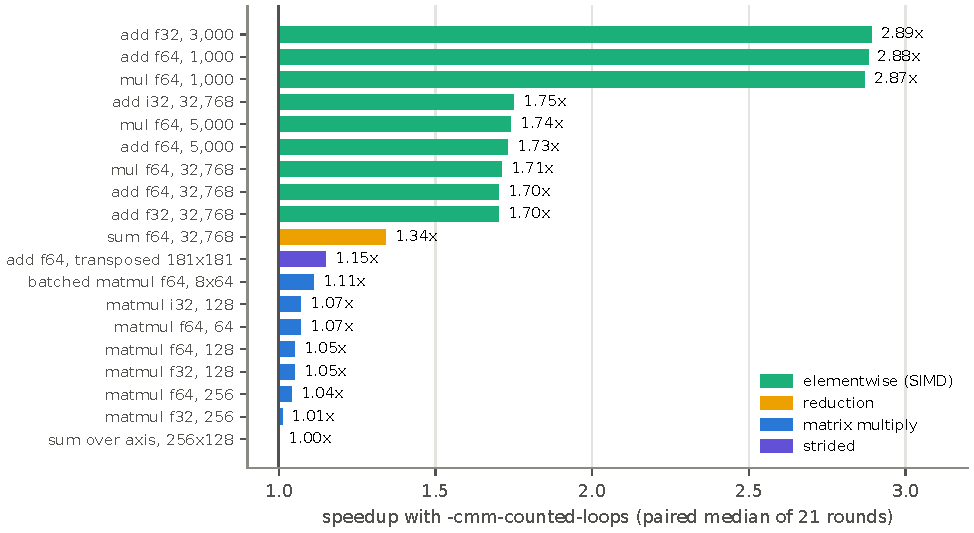
\includegraphics[width=0.86\textwidth]{fig_nx_ops}
  \caption{nx-oxcaml, every benchmarked operation, counted loops versus the same
  compiler without them (21 rounds, polls on in both).}
  \label{fig:nxops}
\end{figure}

The spread follows from what the pass removes. Only 4 of the 22 loop
instructions of an element-wise addition are arithmetic; at 1,000 elements
instruction count sets the speed ($2.9\times$), at 32,768 memory starts to
limit it ($1.7\times$). Matrix multiply is almost pure arithmetic.

This comparison mixes two changes: counted loops remove the back-edge polls,
and the generalised analysis lets the pointer passes act on nx's SIMD loops at
all. A second nx run (21 rounds, identical results in every arm) changes one
thing at a time (Table~\ref{tab:nxablation}). Removing polls with the pointer
passes off measures the polls' own cost: a few percent. The pointer passes in
builds without polls measure the analysis alone: most of the gain. Counted
loops match that poll-free build. The speed-up therefore comes from the
generalised analysis; moving the polls lets it act. With default
flags the final passes run these kernels at the speed of the passes-off build
(Section~\ref{sec:sr-pass}), so counted loops are worth $1.42$--$2.43\times$
over either.

\begin{table}[h]
  \centering
  \small
  \begin{tabular}{@{}lr@{}}
    \toprule
    nx element-wise kernels (9 cases), paired speed-up & range \\
    \midrule
    removing polls, pointer passes off & $1.04$--$1.08\times$ \\
    pointer passes, both builds without polls & $1.60$--$2.58\times$ \\
    counted loops against removing every poll & $0.97$--$1.01\times$ \\
    counted loops against passes off & $1.42$--$2.43\times$ \\
    \midrule
    final passes, defaults against the defaults measured above & $1.10$--$1.14\times$ \\
    final passes, counted loops against counted loops above & $0.99$--$1.01\times$ \\
    \bottomrule
  \end{tabular}
  \caption{What the nx-oxcaml speed-ups are made of (separate 21-round run,
  single domain; two byte-identical builds differed by about 1\%). The last two
  rows are a later 15-round run with the final passes.}
  \label{tab:nxablation}
\end{table}

\subsection{How Close Is Counted to Poll-Free?}
\label{sec:last2}
Removing polls altogether is worth $+1.2\%$ (13/21) over the counted
build (interquartile range $[-0.8, +7.4]\%$), within run W's
resolution (byte-identical copies differ by $+0.6\%$,
$[-0.2, +2.9]\%$).

Of the four polls left in \code{linear} (row-group loop exit, function exit,
fallback copy), each call executes two, never taken, outside every loop.
After normalising addresses, \code{linear}'s 42-instruction row-group loop is
identical to that of a build with no polls. Outside it, the counted build
keeps a stack frame in \code{linear} and carries the fallback loops
(\code{linear} grows from 107 to 215 instructions, \code{forward} from 582 to
777). Overwriting every remaining poll with NOPs (Section~\ref{sec:polls})
changed nothing measurable in a separate test.

The obvious remaining candidate is code layout: if a loop's address alone
moves a build by as much as the builds differ, no difference can be credited
to the polls or to loop versioning. A separate test relinked the counted,
unchecked and poll-free builds at four code addresses each, \code{linear}'s
instructions identical in all twelve (21 rounds). Moving the code changed each
build's speed by 2--3.5\%, while averaged over the four layouts the three
builds differ by at most 0.4\%, and which is fastest depends on the layout.
Counted loops are therefore as fast as removing polls altogether.

\subsection{What Counted Loops Cost}
The final compiler counts 39 of microgpt's 85 loops: 25 proved at compile
time and 14 guarded by an entry check (two copies). The other 46 are rejected:
39 contain a GC point, 6 have no exit test dominating the back edges, and 1
has an inner entry check that could not be lifted. The module's machine code grows
by 2.1\% (58,817 to 60,059 bytes) and the whole binary by 0.07\%. Build time
is unchanged (medians 2.29--2.31\,s over seven interleaved builds).

\section{Stage IX: Explicit SIMD in OxCaml}
\label{sec:simd}

The last remaining difference was vectorisation, so I added an OxCaml kernel
that uses SIMD explicitly (build switch \code{MG_SIMD=1}). Splitting one row's
dot product across lanes would reassociate the sum and break the bit-exact
contract, so the kernel puts \emph{rows} in lanes, each adding the same
products in the same order as the scalar kernel, as GCC's vectoriser does.

\begin{lstlisting}[language=OCamlX,caption={The SSE2 kernel's inner loop. \texttt{F.add} and \texttt{F.mul} are \texttt{[@@builtin]} externals on the unboxed 128-bit type \texttt{float64x2\#}.},label=lst:simd]
let rec go i (v01 : float64x2#) (v23 : float64x2#) =
  if i >= cols then #(v01, v23)
  else
    let xi = unbox x.(i) in
    let xv = F.pair xi xi in                               (* broadcast x.(i) *)
    let r01 = F.pair (unbox d.(b0 + i)) (unbox d.(b1 + i)) in  (* rows 0, 1 *)
    let r23 = F.pair (unbox d.(b2 + i)) (unbox d.(b3 + i)) in  (* rows 2, 3 *)
    go (i + 1) (F.add v01 (F.mul r01 xv)) (F.add v23 (F.mul r23 xv))
\end{lstlisting}

The intrinsics are expanded inline, so no C call happens at run time. All
SIMD builds produce the reference output.

\subsection{Results: SIMD Helps Most Where the Passes Cannot Act}
\label{fig:interaction}
GCC's vectoriser is worth $+9.5\%$ (21/21) to C++. On the
pull-request compiler with the passes off, the SSE2 kernel is worth
$+15.7\%$ (19/21). With the passes on it adds much less:
$+0.9\%$ (12/21) (interquartile range $[-6.9, +7.5]\%$) with a poll on
every back edge, $+1.8\%$ (14/21) with no polls, and
$+5.2\%$ (18/21) with counted loops, leaving OxCaml with the
SSE2 kernel $1.26\times$ behind scalar C++, against $1.29\times$
for the scalar kernel. SIMD and the pointer passes remove
overlapping work.

\subsection{Why SIMD Adds Little to the Passes}
\label{sec:simd-why}
Interior pointers and the shared row index survive in the SIMD kernel
(Listing~\ref{lst:simd-asm}); without the passes it needs four more
\code{lea}s per iteration (20 instructions instead of 16).

\begin{lstlisting}[language=asmX,caption={The SSE2 kernel's inner loop without safepoints: 16 instructions per iteration against the scalar loop's 13, the extra work being packing.},label=lst:simd-asm]
vmovsd   -0x4(%rax,%rbp,4),%xmm2     # x[i]
vmovapd  %xmm2,%xmm3
vmovlhps %xmm2,%xmm3,%xmm2           # broadcast x[i] into both lanes
vmovsd   -0x8(%r10,%rbp,4),%xmm3     # row 0: interior pointer + shared index
vmovsd   -0x8(%r13,%rbp,4),%xmm4     # row 1
vmovlhps %xmm4,%xmm3,%xmm3           # pack (row 0, row 1)
vmovsd   -0x8(%r12,%rbp,4),%xmm4     # row 2
vmovsd   -0x8(%r9,%rbp,4),%xmm5      # row 3
vmovlhps %xmm5,%xmm4,%xmm4           # pack (row 2, row 3)
vmulpd   %xmm2,%xmm4,%xmm4
vaddpd   %xmm4,%xmm0,%xmm0           # accumulators for rows 2, 3
vmulpd   %xmm2,%xmm3,%xmm2
vaddpd   %xmm2,%xmm1,%xmm1           # accumulators for rows 0, 1
add      $0x2,%rbp
cmp      %rbx,%rbp
jl       .loop
\end{lstlisting}

One row's elements are not adjacent to the next row's, so the kernel issues
the same five scalar loads and spends three shuffles and a move packing them,
in exchange for halving the floating-point instructions. It also has only two
accumulators where the scalar kernel has four independent chains.

If each loop is limited by its chains of dependent additions, doubling the
chains should speed up both kernels; if by the floating-point ports, extra
chains change nothing for the scalar kernel, while the SSE2 kernel, with half
as many operations, may be chain-limited. An eight-row version of both
kernels tests this (a separate 21-round run, identical output). Extra rows
barely help the scalar kernels ($+3.8\%$ for C++, nothing for OCaml), as a
port-limited loop predicts. The SSE2 kernel, now with four vector accumulators, gains $+5.1\%$
over its four-row version and beats the eight-row scalar kernel by $+4.7\%$
(21/21 rounds, with counted loops), where at four rows the two were equal in
that run. The
scalar loop is therefore port-limited, as the model of
Section~\ref{sec:residual} also finds, and the four-row SSE2 kernel
chain-limited.

In the counted build's hot copy of the SIMD loop, the fallback copy's live
values push three of the four interior pointers onto the stack (19
instructions): SIMD and interior pointers compete for registers. SIMD is the right tool where
the passes cannot act; with counted loops it adds a few percent, and the
scalar kernel, simpler and free of OxCaml extensions, gets most of the way.

\section{Where the Optimisations Do and Do Not Apply}
\label{sec:generality}

nx-oxcaml shaped the generalised analysis of Section~\ref{sec:counted}, so it
is a development workload, not an independent test. Two workloads the passes
were not adjusted for follow: a standard kernel suite, which gains, and a
cryptography code base, which does not. A port of the passes to stock OCaml
comes first.

\subsection{The Passes on Stock OCaml 5.3.0}
\label{sec:stock}
None of the passes depends on flambda2, so I ported them to OCaml 5.3.0.
Stock OCaml polls every loop, so with default flags only strength reduction
fires: the passes gain $+12.2\%$ (21/21) on microgpt. Counted
loops add $+4.9\%$ (17/21), for
$+17.6\%$ (21/21) in all over stock OCaml, and the
inner loop goes from 30 to 17 instructions per 4 multiply--adds. The best OxCaml build stays $+12.8\%$ (20/21)
ahead of the best OCaml build. OCaml's test suite (1,462 tests) gives the same
result test by test with and without the patches, also with counted loops
forced on.

\subsection{A Held-Out Kernel Suite: PolyBench}
\label{sec:polybench}
PolyBench/C~\cite{polybench} is a standard suite of loop-nest kernels
(linear algebra, stencils, data mining) written by others for compiler
research. I ported 17 of its kernels to plain OCaml as an ordinary programmer
would write them (flat row-major \code{float array}s, \code{for} loops,
\code{-unsafe}) and to C, and ran them on the pull-request compiler in a
separate 21-round run. All builds produce bit-identical results, and all
84 loops in the timed kernels are counted (Table~\ref{tab:polybench}). The
geometric-mean gain is $+19.7\%$ with array sizes fixed at compile time
(gemm $+108\%$) and $+7.5\%$ with sizes known only at run time. The
rules of Table~\ref{tab:applicability} predict that kernels whose inner loops
index arrays as \code{base + m*counter + c} should gain, and kernels limited by
memory bandwidth or a chain of dependent arithmetic should not.

\begin{table}[h]
  \centering
  \small
  \begin{tabular}{@{}lrrr@{}}
    \toprule
    kernel & counted loops vs passes off & inner-loop instructions & gap to scalar C \\
    \midrule
    gemm & $+108.2\%$ (21/21) & 19 $\to$ 8 & $2.24\times$ \\
    jacobi-2d & $+49.6\%$ (21/21) & 21 $\to$ 11 & $1.43\times$ \\
    fdtd-2d & $+48.7\%$ (21/21) & 18--22 $\to$ 10--12 & $1.34\times$ \\
    syrk & $+42.6\%$ (21/21) & 20 $\to$ 11 & $2.34\times$ \\
    doitgen & $+33.5\%$ (21/21) & 21 $\to$ 11 & $3.16\times$ \\
    floyd-warshall & $+26.2\%$ (21/21) & 23 $\to$ 15 & $2.12\times$ \\
    heat-3d & $+16.6\%$ (21/21) & 38 $\to$ 31 & $1.49\times$ \\
    atax & $+15.0\%$ (20/21) & 15 $\to$ 7 & $2.26\times$ \\
    2mm & $+10.5\%$ (20/21) & 19 $\to$ 11 & $3.65\times$ \\
    8 others & $-0.7$ to $+6.4\%$ & & $1.18$--$2.84\times$ \\
    \midrule
    geometric mean, 17 kernels & $+19.7\%$ & & $2.03\times$ \\
    \quad same 17 kernels, sizes known only at run time & $+7.5\%$ & & \\
    \bottomrule
  \end{tabular}
  \caption{PolyBench in plain OCaml with \texttt{-unsafe}: the passes with
  counted loops against the passes off, polls on in both (paired median,
  rounds won; sizes fixed at compile time unless noted). Two
  byte-identical builds differed by $-0.5$ to $+2.1\%$ per kernel. Others:
  gemver, trmm, mvt, gesummv, bicg, seidel-2d, covariance, correlation.}
  \label{tab:polybench}
\end{table}

The prediction holds. Gains are large where an inner loop indexes several
two-dimensional arrays this way (gemm, the stencils, syrk, doitgen) and the
passes remove most of its instructions, which counted loops allow by moving
the poll to the exit. Gains are small where something else
limits the loop: matrix--vector kernels on 32--64\,MB matrices that wait on
memory, column-strided access, and seidel-2d, whose loop shrinks from 37 to 15
instructions for only $+2\%$ because each update waits for the previous one.

Two further results bound the claim. With sizes known only at run time the
gain is $+7.5\%$: constant sizes let the compiler fold each row stride into
the loop,
while run-time strides stay as multiplications inside it and add register
pressure, so the passes remove a smaller share of its work (gemm's
loop shrinks from 30 to 27 instructions instead of 19 to 8). And OCaml stays
$2.03\times$ behind scalar C, because GCC keeps array-element accumulators in
registers and unrolls and interleaves the gemm loop, which no OCaml pass does.

\subsection{The oxcaml-crypto-study Repository}
\label{sec:crypto}
oxcaml-crypto-study~\cite{crypto_study} asks whether OxCaml can implement
cryptographic primitives natively, at Rust-like speed, instead of binding to C.
Its one primitive, ChaCha20~\cite{rfc8439}, exists as a boxed plain-OCaml
version and an OxCaml version with unboxed \texttt{int32\#} arrays,
stack-allocated state and \code{[@zero_alloc]}. I compiled both with the
pull-request compiler in eight configurations (the polling modes, each with
and without the pointer passes) and timed encryption of 1\,MiB\,+\,37 bytes
over 15 interleaved rounds; all passed the RFC~8439 test vector.

\subsection{Result: No Measurable Effect}
In every polling mode the assembly is \emph{byte-identical} with the four
passes on or off; the flags only drop back-edge polls in nine loops. The best
configuration measured $\times1.019$ (12/15 rounds), while two byte-identical
builds differed by 1.7\%, for four reasons:

\begin{enumerate}
  \item \textbf{Byte offsets, not array elements.} The hot XOR loop's
        \code{Bytes.get_int32_le plaintext (j*64 + i*4)} untags a byte offset
        with a \emph{right} shift and adds it unscaled; the passes match
        addresses scaled by a left shift.
  \item \textbf{The invariant is not a variable.} flambda2 inlines
        \code{j * 64} into the address as \code{(<< j 6)}; writing
        \code{let base = j * 64} gave byte-identical assembly.
  \item \textbf{The other loops are already optimal or not GC-free.} The copy
        and add loops index by the bare counter, the round loop calls a
        non-inlined function, and the boxed version allocates on every store.
  \item \textbf{The ceiling is low.} Each block makes 80 calls to a
        94-instruction quarter-round, about 7,500 instructions, against
        roughly 600 in loops the passes could touch.
\end{enumerate}

\subsection{An Applicability Characterisation}
Table~\ref{tab:applicability} summarises the results: the passes recover
C-style pointer walking over arrays, helping code whose cost is index
arithmetic and doing nothing for code whose cost is the computation itself.

\begin{table}[h]
  \centering
  \small
  \begin{tabularx}{\textwidth}{@{}lXX@{}}
    \toprule
    property & benefits & does not benefit \\
    \midrule
    addressing & array index \code{base + m*counter + c}, scaled by a left shift & byte offsets into \code{Bytes}; an index that is the bare counter \\
    invariant part & a variable bound before the loop, or a loop-invariant stride & an invariant product inlined into the address \\
    GC-freedom & no allocation or non-inlined call; polls moved to exits by counted loops & loops that call functions or box values \\
    where time goes & inner loops dominated by address arithmetic & arithmetic reached through calls; compute-bound kernels \\
    registers & free registers for the carried pointers & loops at the register limit \\
    \bottomrule
  \end{tabularx}
  \caption{When the Cmm loop passes apply.}
  \label{tab:applicability}
\end{table}

A vectorised ChaCha20, or number-theoretic transforms indexing
\code{a.(j + len)}, have the shapes the passes handle.

\section{Summary of Results}
\label{sec:results}

Figure~\ref{fig:ladder} puts the whole evolution on one axis.

\begin{figure}[h]
  \centering
  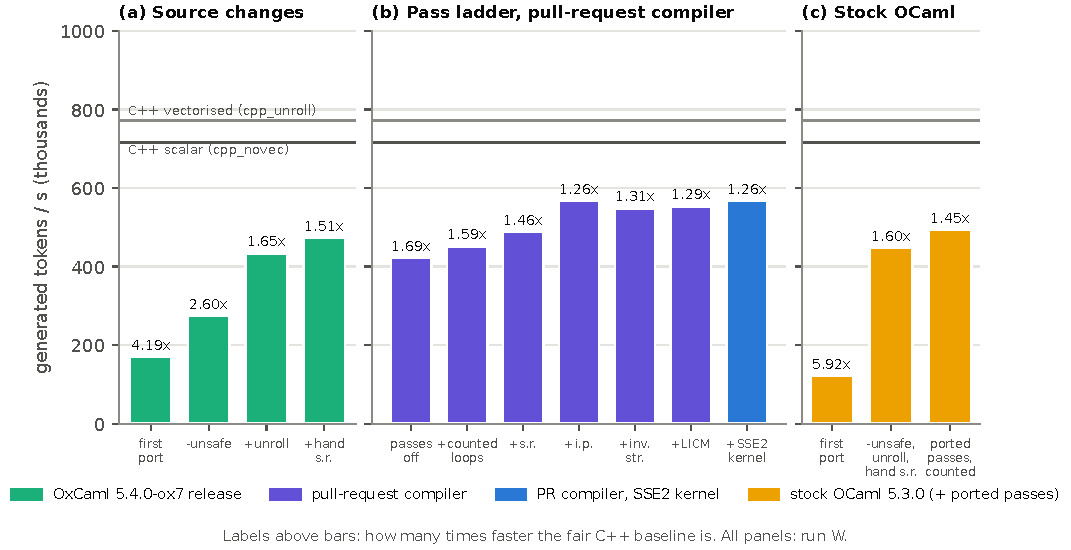
\includegraphics[width=\textwidth]{fig_gap_ladder}
  \caption{Closing the gap (run W): scalar C++ throughput over each OCaml
  variant's. Every build keeps its polls (on back edges, or at loop exits with
  counted loops). The SSE2 bar adds one change to the last ladder step.
  Abbreviations: s.r., strength reduction; i.p., interior pointers;
  inv.\ str., invariant-stride induction variables.}
  \label{fig:ladder}
\end{figure}

\subsection{Every Final Configuration}
\label{sec:unified}

\begin{table}[h]
  \centering
  \small
  \begin{tabularx}{\textwidth}{@{}Xrrr@{}}
    \toprule
    configuration (same OCaml source unless noted) & tokens/s & vs scalar C++ & vs vectorised C++ \\
    \midrule
    C++ vectorised (\code{cpp_unroll}) & 772,261 & $0.93\times$ & $1.00\times$ \\
    C++ scalar (\code{cpp_novec}) & 716,505 & $1.00\times$ & $1.08\times$ \\
    Rust (\code{rust_unroll}, bounds-checked) & 703,295 & $1.02\times$ & $1.10\times$ \\
    \midrule
    stock OCaml 5.3.0, first port (\code{ocaml_safe_plain}) & 121,019 & $5.92\times$ & $6.38\times$ \\
    \quad \code{-unsafe}, unrolled, hand s.r.\ (\code{ocaml_unsafe_sr}) & 448,265 & $1.60\times$ & $1.72\times$ \\
    \quad \code{-unsafe}, unrolled, ported passes + counted loops (\code{ocaml_pr_counted}) & 493,014 & $1.45\times$ & $1.57\times$ \\
    \midrule
    OxCaml 5.4.0-ox7 release, first port (\code{oxcaml_safe_plain}) & 170,978 & $4.19\times$ & $4.52\times$ \\
    \quad \code{-unsafe}, unrolled (\code{oxcaml_unsafe_unroll}) & 433,992 & $1.65\times$ & $1.78\times$ \\
    \quad + hand s.r.\ (\code{oxcaml_unsafe_sr}) & 473,779 & $1.51\times$ & $1.63\times$ \\
    \midrule
    PR compiler, \code{-unsafe}, unrolled, passes off (\code{pr_off}) & 423,171 & $1.69\times$ & $1.82\times$ \\
    \quad all passes + \code{-cmm-counted-loops} (\code{pr_counted}) & \textbf{553,383} & \textbf{$1.29\times$} & \textbf{$1.40\times$} \\
    \quad + SSE2 kernel (\code{pr_simd_counted}) & 567,161 & $1.26\times$ & $1.36\times$ \\
    \midrule
    bounds checks kept: release, unrolled (\code{oxcaml_safe_unroll}) & 348,459 & $2.06\times$ & $2.22\times$ \\
    \quad PR compiler, all passes + counted loops (\code{pr_safe_counted}) & 292,970 & $2.45\times$ & $2.64\times$ \\
    \bottomrule
  \end{tabularx}
  \caption{The core configurations in run W (generation mode, median of 21
  interleaved rounds; ratios are C++ throughput over the variant's; s.r.,
  strength reduction). All rows but the first ports and the last two use
  \code{-unsafe}; the headline is the scalar \code{pr_counted} row, and the
  SSE2 row adds an explicitly vectorised kernel. Close builds can be ordered differently here than by
  the paired comparisons, which are the reliable ones. Scoring mode agrees on
  every difference larger than the resolution.}
  \label{tab:final}
\end{table}

Beyond Table~\ref{tab:final}, paired comparisons settle three questions:

\begin{itemize}
  \item \textbf{Counted loops carry the gain:} $+16.6\%$ (21/21)
        over the four passes with a poll on every back edge, and with the
        passes $+30.2\%$ (21/21) over passes off
        ($+31.0\%$ (21/21) in scoring mode), and
        $+29.2\%$ (21/21) over the release; the price is
        pause latency (Section~\ref{sec:counted}).
  \item \textbf{The gain needs the pointer passes:} within counted mode they
        are worth $+13.3\%$ (21/21); moving polls to loop exits
        matters because it makes the pointers legal.
  \item \textbf{Counted loops are as fast as poll-free code} within the run's
        resolution, $+1.2\%$ to no polls at all
        (Section~\ref{sec:last2}); unchecked loops and the other builds that
        give up liveness gain no more than about the resolution
        (Table~\ref{tab:liveness}).
\end{itemize}

\paragraph{With bounds checks kept.} Every OCaml figure above except the
first ports uses \code{-unsafe}; Rust keeps its bounds checks and is
$1.02\times$ behind C++. With checks kept, the pull request is
\emph{slower} than the release: $-14.9\%$ (1/21) against
bounds-checked OxCaml, $2.45\times$ behind C++, and
$-47.2\%$ (0/21) against the counted build without checks.
Interior pointers still form, but each check needs the row's index as well as
its pointer: with eight values live instead of four, the allocator spills and
reloads the four row pointers every iteration. I did not build a fix.

\subsection{Does the Gap Survive a Wider Model?}
\label{sec:width}
microgpt's weights fit in the L1 data cache (Section~\ref{sec:model}). A
sweep (a separate run, 21 interleaved rounds) widened the model, with no code
change, to one layer, four heads and widths of 16 to 256, taking the weights
through L2 (116\,KB--1.6\,MB) into L3 (6.4\,MB); all variants agree on every
model's output. The wider models have random weights, which generate names
about twice as long, so attention does more work per token; at width 16 that
alone moves the counted build from $1.24\times$ to $1.42\times$ behind scalar
C++. Widths are therefore compared among random models
(Figure~\ref{fig:width}).

\begin{figure}[h]
  \centering
  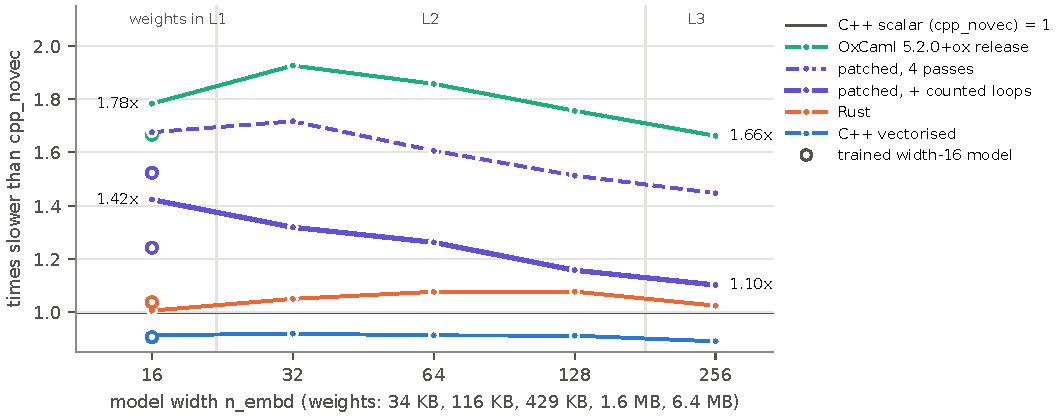
\includegraphics[width=\textwidth]{fig_width}
  \caption{The gap to scalar C++ as the model widens (width-sweep run, one
  layer, 21 rounds, median tokens/s). Lines are models with random weights;
  the open markers are the trained width-16 model. The patched compiler with
  counted loops polls at loop exits.}
  \label{fig:width}
\end{figure}

With counted loops, OxCaml goes from $1.42\times$ behind scalar C++ at width
16 to $1.32\times$ at 32, $1.26\times$ at 64, $1.16\times$ at 128 and
$1.10\times$ at 256 (C++ won at least 20 of 21 rounds at every width); the
5.2.0+ox release build stays $1.66$--$1.93\times$ behind. At widths 32--256
counted loops gain $+46$ to $+51\%$ over that build and $+27$ to $+31\%$ over
the four passes alone (paired medians, at least 20/21 rounds each).

Why does the gap narrow? If memory is the cause, the ratio should narrow only
when the weights stream from a slower level; if the shape is the cause
(longer rows spreading each row's setup over more multiply--adds), it should
narrow with matrix size even in cache. A separate micro-benchmark of the
four-row kernel, with the weights reused (in cache) or cycled through 8\,MB
(L3) or 64\,MB (main memory), decides it. The OCaml/C++ ratio falls from
$1.19\times$ at $16\times16$ to $1.07$--$1.14\times$ at $256\times256$ and
larger in cache, and no further from L3; only from main memory, which no
model reaches, do the two converge. The narrowing therefore follows the loop
shape: longer rows amortise the setup that Section~\ref{sec:residual} places
outside the inner loop. GCC's vectoriser stays worth 8--10\% at every width,
and Rust within 1--7\% of scalar C++.

\subsection{In Words}
Source-level work took OxCaml from $4.19\times$ to
$1.65\times$ behind scalar C++. The compiler work, on unchanged
source, closed more than half of the remaining gap, to $1.29\times$ with
counted loops ($1.40\times$ behind vectorised C++).
Figure~\ref{fig:matrix} shows every core build of run W.

\begin{figure}[t]
  \centering
  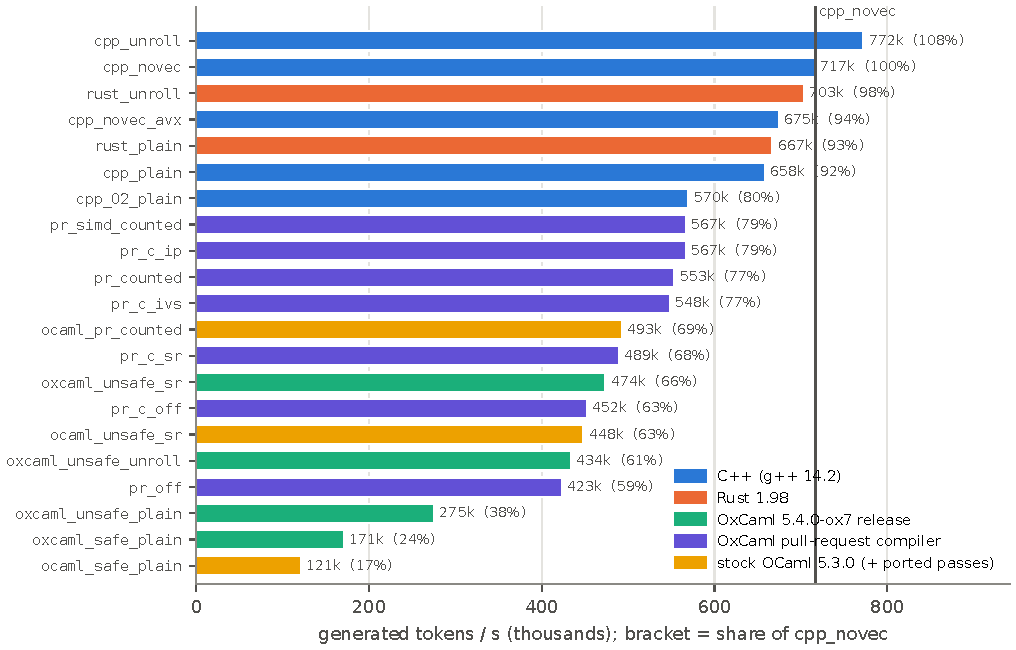
\includegraphics[width=\textwidth]{fig_matrix}
  \caption{The core builds of run W (median of 21 interleaved rounds; Python,
  6,479 tokens/s, is omitted). \texttt{oxcaml\_*} builds use the
  5.4.0-ox7 release and \texttt{pr\_*} the pull-request compiler
  (Section~\ref{sec:method}).}
  \label{fig:matrix}
\end{figure}

\section{Notable Engineering Challenges}
\label{sec:challenges}

\subsection{Challenge 1: Keeping the Reference Arithmetic Identical}
CPython's compensated \code{sum()} (Table~\ref{tab:bugs}) changed the weight
checksum by only $5\times10^{-15}$ relative and left the generated text
unchanged. Comparing outputs cannot reveal such a difference; checking each
port against the numerical contract can, and checksums are compared exactly.

\subsection{Challenge 2: Measuring on a Hybrid Laptop}
Without care, ratios on a hybrid laptop vary by almost $3\times$ between runs,
and subtler effects bias a comparison: perplexity run after generation in the
same process slows 1.5 times, and C++ at \code{-O2} against Rust at opt-level
3 favours Rust by 20\%. The protocol of Section~\ref{sec:method}, explicit
compiler paths, and requiring the two modes to agree make such effects
visible.

\subsection{Challenge 3: Testing Each Explanation}
Each plausible explanation became a prediction measured before it was used:
the gap is not SIMD (Section~\ref{sec:stage2}), the poll's cost is not the
\reg{r11} spill (Section~\ref{sec:r11}), and nx-oxcaml's kernels were limited
by address arithmetic, not memory (Section~\ref{sec:counted}).

\subsection{Challenge 4: Keeping the Gains With Safepoints}
The pointer passes need loops without polls, and the release configuration
puts a poll on every back edge (Section~\ref{sec:reality}). Measured only on
compilers built without polls, the passes would overstate what users get.
Counted loops recover the gain while keeping the collector safe and every
proved loop reaching a poll: polls move to loop exits, and the cost is pause
latency, which an optional trip cap bounds in iterations, not in time.

\subsection{Challenge 5: Keeping Pointer Optimisations Safe}
The \code{bad GC root} check, which turns any derived pointer live at a
safepoint into a compile-time error, shaped the design: it rules out carrying
a pointer across a nested loop's poll, a polled loop inside a counted loop's
entry check, and exit polls in the runtime's never-polled helpers. What no
compile-time check catches, a loop waiting on another domain, counted loops
exclude by requiring a termination proof; unchecked mode handles only some
such loops, so it stays opt-in (Section~\ref{sec:counted}).

\section{Conclusions and Future Work}
\label{sec:conclusion}

\begin{itemize}
  \item \textbf{Correctness first.} Five ports give the same text and the same
        perplexity in all 17 printed digits, which took a written numerical
        contract and an output hash; matching text alone proves little.
  \item \textbf{Most of the first gap was ordinary:} bounds checks and missing
        instruction-level parallelism, whose value depended on how well each
        compiler's plain loop already ran.
  \item \textbf{The rest was integer bookkeeping, not floating point and not
        SIMD.} OCaml's ban on interior pointers forces index arithmetic, and
        Cmm passes remove it without changing the source, with derived
        pointers confined to loop regions in which no object can move.
  \item \textbf{Safepoints are the real constraint.} Counted loops move polls
        to loop exits, keeping the collector safe and every proved loop
        reaching a poll, at the cost of unbounded pause latency, and
        let the passes act: $+30.2\%$ (21/21) on unchanged source,
        leaving OxCaml $1.29\times$ behind scalar C++ with bounds checks
        off ($1.26\times$ with the SSE2 kernel); with bounds checks
        kept the pull request is $-14.9\%$ (1/21)
        against the release.
  \item \textbf{The passes generalise to loops of a precise shape,} arrays
        indexed as \code{base + m*counter + c}, as the held-out PolyBench
        kernels and the port to stock OCaml confirm; they do nothing for
        compute-bound or call-heavy code such as ChaCha20.
  \item \textbf{What remains is not instruction count.} The patched inner loop
        is, by \code{llvm-mca}'s model, limited by the floating-point ports,
        like C++'s; by an estimate from isolated timings, about half of the
        remaining gap lies outside it, and longer rows shrink it.
  \item \textbf{Explicit SIMD and the passes overlap:} with counted loops the
        SSE2 kernel adds only $+5.2\%$.
\end{itemize}

The broader point matches my guide's framing: to get performance from OxCaml
you opt in --- with \code{-unsafe}, explicit SIMD, or a flag such as
\code{-cmm-counted-loops} --- and the compiler meets you most of the way.

\subsection{Limitations}
\begin{itemize}
  \item \textbf{Bounds checks.} With checks kept, the pull request is slower
        than the release (Section~\ref{sec:unified}).
  \item \textbf{Latency.} A counted loop delays other domains'
        stop-the-world requests for its whole running time; the trip cap that
        bounds this is off by default, limits iterations rather than time,
        and costs microgpt much of its gain.
  \item \textbf{One target.} Only x86-64 was tested; arm64 and the LLVM
        backend are untested.
  \item \textbf{One small model.} Every microgpt conclusion rests on one
        34\,KB model, and the width sweep used one layer, random weights and a
        short context; deeper and attention-heavy models are untested.
  \item \textbf{Resolution.} Run W resolves about 3\%; counted, unchecked and
        poll-free builds differ by about that much or less, and on some nx
        cases code placement alone moves results by up to about 12\%.
\end{itemize}

\subsection{Future Work}
\begin{itemize}
  \item \textbf{Bounded latency:} strip mining, counted strips inside a polled
        outer loop, as C2 does.
  \item \textbf{Bounds-checked code:} decline interior pointers where a check
        keeps the index live, or replace the test with the pointer (linear
        function test replacement).
  \item \textbf{Upstreaming:} split the pull request, starting with strength
        reduction; test on arm64; resolve the \reg{r11} question.
  \item \textbf{Attribute the last gap} with \code{perf stat}, and measure
        wider programs with Sandmark.
  \item \textbf{Derived pointers across safepoints:} frame-table entries that
        rebuild a derived pointer from its
        base~\cite{diwan1992compiler,llvm_statepoints}.
  \item \textbf{Larger workloads:} deeper models, the attention
        restructuring of Section~\ref{sec:residual}, and calling an OxCaml hot
        loop from \code{llama.cpp} through the foreign function interface, as
        my guide suggested.
\end{itemize}


\clearpage
\phantomsection
\addcontentsline{toc}{section}{References}
\markboth{References}{}
\bibliographystyle{plain}
\bibliography{references}

\end{document}
